\section{Composite Finite Element Analysis}

\indent

The \textit{ANSYS Composite PrepPost} finite element package was used predict the load-bearing capacity and failure behavior of the FDM CFRP bridge specimen. Solid-body FEA of aluminum and ABS bridge bodies were also performed for comparison and model validation. This appendix rigorously details the setup and program options used to develop these finite element models. The ANSYS Composite PrepPost User's Guide was used to learn ACP tools \cite{ACP-manual}.\\

\subsection{Physics Models}

\indent

Figure~\ref{fig:fea-project-schematic} shows the project schematic for the FDM CFRP FEA. The geometry is first imported from \emph{SolidWorks} into \emph{ANSYS Workbench}. An \textit{ACP (Pre)} block is created and references the imported geometry.\textit{ACP (Pre)} is used to establish orthotropic material properties, stackups, layups, laminates, and shell element thickness(es). This data is then transfered to a standard \textit{Static Structural} analysis, where the geometry is descritized using a mesh and loads and boundary conditions are applied to the geometry. A solid-body orthotropic analysis can be performed at this stage and outputs standard result sets, such as Von Mises stresses, but will not contain any composite-specific failure behavior. Consequently, the data from \textit{Static Structural} is exported to yet another \textit{ACP (Pre)} block and to an \textit{ACP (Post)} block. The second \textit{ACP (Pre)} block now accesses mesh data. With the mesh now included in the ACP finite element model, oriented element sets, reference direction, fiber orientation, and solid model representations can be created prior to solving. While no line directly connects the \textit{ACP (Pre)} and \textit{ACP (Post)} blocks in the schematic, \textit{ACP (Post)} pulls all of the ACP setup and loads information to perform its analysis. Contour plots of results, such as deformation and failure behavior, are created. For the purpose of this analysis that is it. In more advanced composite analyses, ACP can paramtrize fiber orientation from 0$^{\circ}$ to 180$^{\circ}$ and iterate between the two to solve for the strongest and or stiffest configuration.\\

\begin{figure}[htp]
\centering
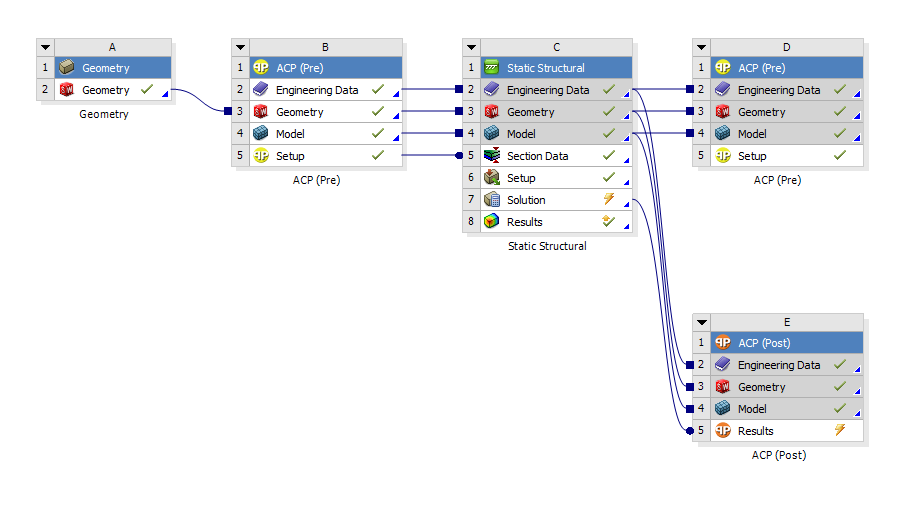
\includegraphics[width=1\textwidth]{./figures/fea/fea-project-schematic}
\caption{A schematic of the physics models used in this FEA.}
\label{fig:fea-project-schematic}
\end{figure}

\clearpage

\subsection{Material Data}

\indent

Table~\ref{tab:ansys-material-properties} lists the materials used in the FEA study. Note that the composite study requires orthotropic elasticities, strain limits, and stress limits. Y and Z-directed properites were assigned values associated with the matrix material, ABS.XY, YZ, and XZ properties were given purely ABS values to create a conservative analysis \large{textbf{CITE}}.\footnote{Carbon fiber and ABS material properties were found from the following websites: \url{http://plastics.ulprospector.com/generics/1/c/t/acrylonitrile-butadiene-styrene-abs-properties-processing}, \url{http://teststandard.com/data_sheets/ABS_Data_sheet.pdf}, and \url{http://www.stratasys.com/~/media/en/Materials/FDM/PC\%20ABS/pc_abs_spec_sheet.pdf}}.\\ Most X-directed properties were assigned values associated with carbon fiber, but \textit{Young's Modulus X Direction}, \textit{Tensile X Direction Stress Limit}, and \textit{Tensile X Direction Strain Limit} were given values found in first-semester filament testing \large{textbf{CITE}}. Since these three values reflect the properties of a CFRP, the analysis is less likely to inflate the predicited strength of the FDM part, which could happen if purely carbon fiber properties were plugged in. Composite failure-specific properties, in this case Puck factors, are also inputs. However, as a phenomenological failure mode, the Puck factors tabulated in Table~\ref{tab:ansys-material-properties} are not material specific. Instead, default values, which have been experimental proven to hold true for most UD CFRP parts, are used.\\

\begin{table}[htp]
    \centering
    \begin{tabular}{lcc}
        Property & Value & Unit \\ \hline
        
        Density & 800 & kg m$^{-3}$\\ 
        
        Young's Modulus X Direction & 2.31E+11 & Pa\\
        Young's Modulus Y Direction & 1.72E+09 & Pa\\
        Young's Modulus Z Direction & 1.72E+09 & Pa\\
        Poisson's Ratio XY & 0.35 &\\
        Poisson's Ratio YZ & 0.35 &\\
        Poisson's Ratio XZ & 0.35 &\\
        Shear Modulus XY & 7E+08 & Pa\\
        Shear Modulus YZ & 7E+08 & Pa\\
        Shear Modulus XZ & 7E+08 & Pa\\
        
        Tensile X Direction Stress Limit & 3.13E+08 & Pa\\
        Tensile Y Direction Stress Limit & 3.45E+07 & Pa\\
        Tensile Z Direction Stress Limit & 3.45E+07 & Pa\\
        Compressive X Direction Stress Limit & -1.57E+08 & Pa\\
        Compressive Y Direction Stress Limit & -1.73E+07 & Pa\\
        Compressive Z Direction Stress Limit & -1.73E+07 & Pa\\
        Shear XY Stress Limit & 6E+07 & Pa\\
        Shear YZ Stress Limit & 3.2E+07 & Pa\\
        Shear XZ Stress Limit & 6E+07 & Pa\\
        
        Tensile X Direction Strain Limit & 0.03 &\\
        Tensile Y Direction Strain Limit & 0.25 &\\
        Tensile Z Direction Strain Limit & 0.25 &\\
        Compressive X Direction Strain Limit & -0.015&\\
        Compressive Y Direction Strain Limit & -0.125 &\\
        Compressive Z Direction Strain Limit & -0.125 &\\
        Shear XY Strain Limit & 0.012 &\\
        Shear YZ Strain Limit & 0.011 &\\
        Shear XZ Strain  Limit & 0.012 &\\  
        
        Puck Material Classification & Carbon &\\
        Puck Compressive Inclination XZ & 0.3 &\\
        Puck Compressive Inclination YZ & 0.25 &\\
        Puck Tensile Inclination XZ & 0.35 &\\
        Puck Tensile Inclination YZ & 0.25 &\\
        
        Puck Interface Weakening Factor & 0.8 &\\
        Puck Degradation Parameter s & 0.5 &\\
        Puck Degredation Parameter M & 0.5 &\\
              
        
    \end{tabular}
    \caption{CFRP material properties used in \textit{ANSYS}.}
    \label{tab:ansys-material-properties}
\end{table}

\clearpage

\subsection{Geometry}

\indent

Figure~\ref{fig:fea-surface-geometry} shows a \textit{SolidWorks} drawing of the surface used for composite FEA. For the purpose of this study, a compressive load will be placed on the outer edges to induce a bending moment on the central arc. Fillets, which minimize stress concentrations, are featured on both sides to ensure that the tendency towards failure is localized to the central arch.\\

\begin{figure}[htp]
\centering
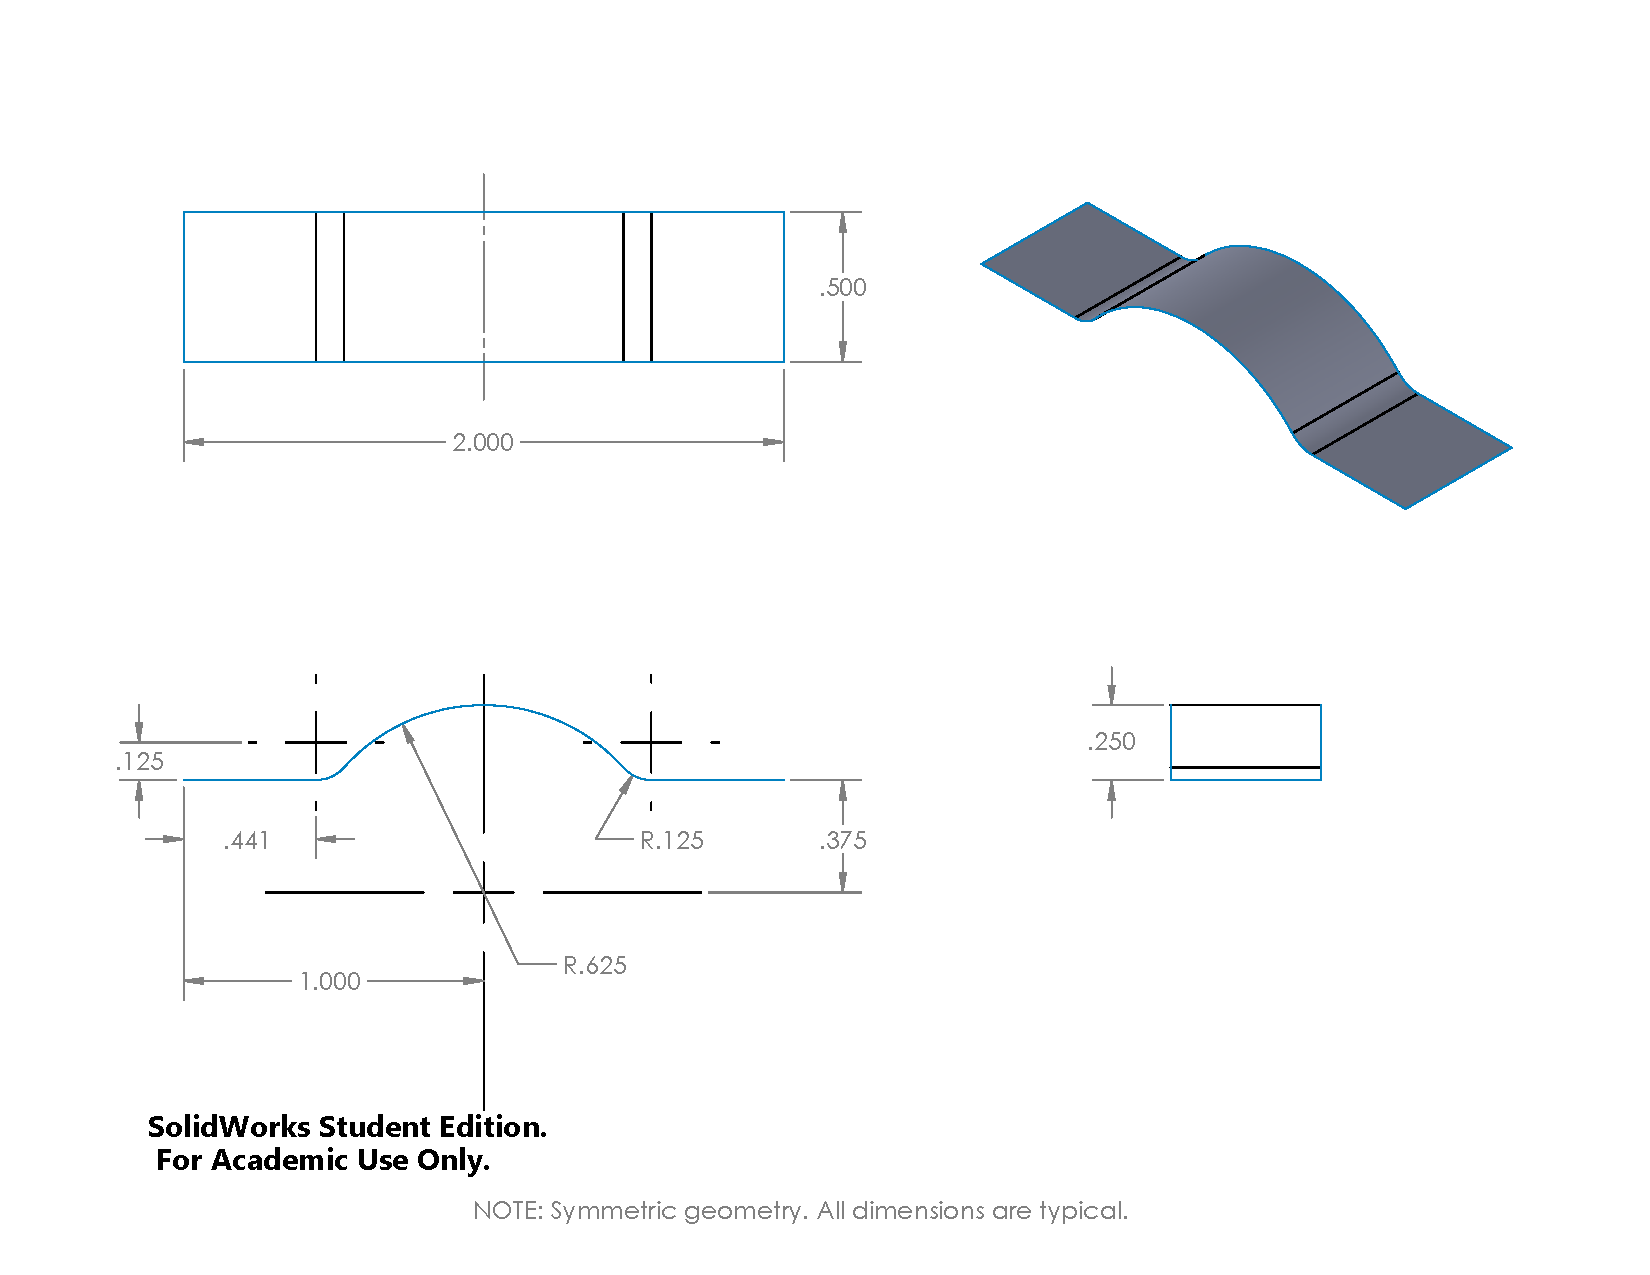
\includegraphics[width=1\textwidth]{./figures/fea/fea-surface-geometry}
\caption{A \emph{SolidWorks} drawing of the surface used for composite FEA.}
\label{fig:fea-surface-geometry}
\end{figure}

\subsection{Loads and Boundary Conditions}

\indent

Figure~\ref{fig:fig:fea-loads-bcs} shows the loads and boundary conditions applied to the geometry, which are designed to mimic a compression tests in Cooper's Instron Tension Tester where both flat faces are gripped in jaws. Subsequently, Edge A is fixed and the opposite edge, B, is experiencing the compressive force (which in this case was found to be a maximum of 90 pounds-force). Zero z-displacement conditions were placed on the flat faces to simulate the gripper jaws. Note that this boundary conditions still leaves x and z diaplacement as free.\\

\begin{figure}[htp]
\centering
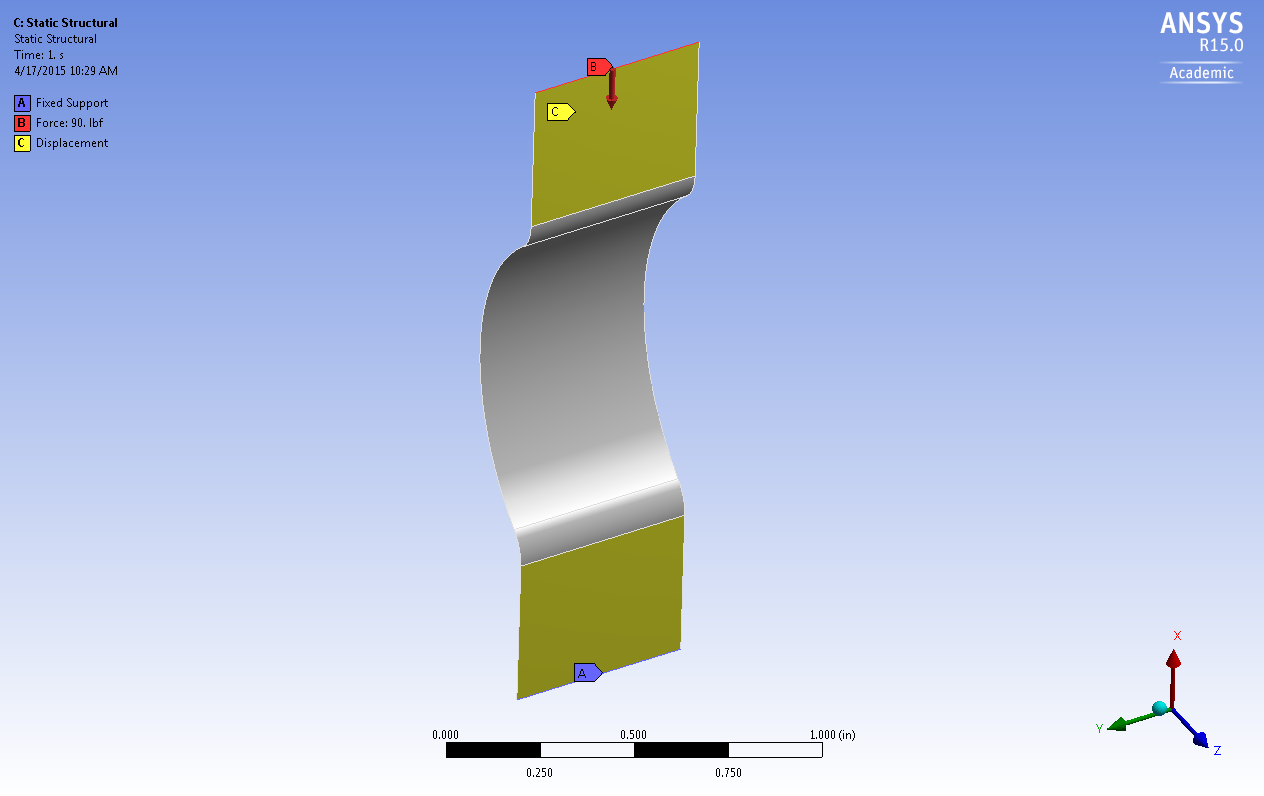
\includegraphics[width=1\textwidth]{./figures/fea/fea-mechanical-loads-bc}
\caption{The loads and boundary conditions applied to the surface geometry.}
\label{fig:fea-loads-bcs}
\end{figure}

\clearpage

\subsection{Meshing}

\indent

Figure~\ref{fig:fea-mechanical-mesh-surface} shows an overview of the meshed surface. Figure~\ref{fig:fea-mechanical-mesh-closeup} shows a close up of the mesh along its smallest feature. A global mesh size constraint of 1/128 inches was placed on the surface in order to discretize the smallest fillet into at least three elements. By using small, second order elements, the model is given a reasonable number of nodes along its smallest feature, which ensures that the analysis will not undershoot the stress values in the smallest geometric features. Figure~\ref{fig:fea-mechanical-mesh-metrics-histogram} shows a mesh statistics histogram focusing on the aspect ratio. Note that the aspect ratio of all elements is almost unity, indicating that the elements are equally weighted (lacking of a relatively stiff direction). Finally, Figure~\ref{fig:fea-mechanical-mesh-thick-shell} shows a thick shell representation of the mesh, which shows the boundaries of all the integration points.\\


\begin{figure}[htp]
\centering
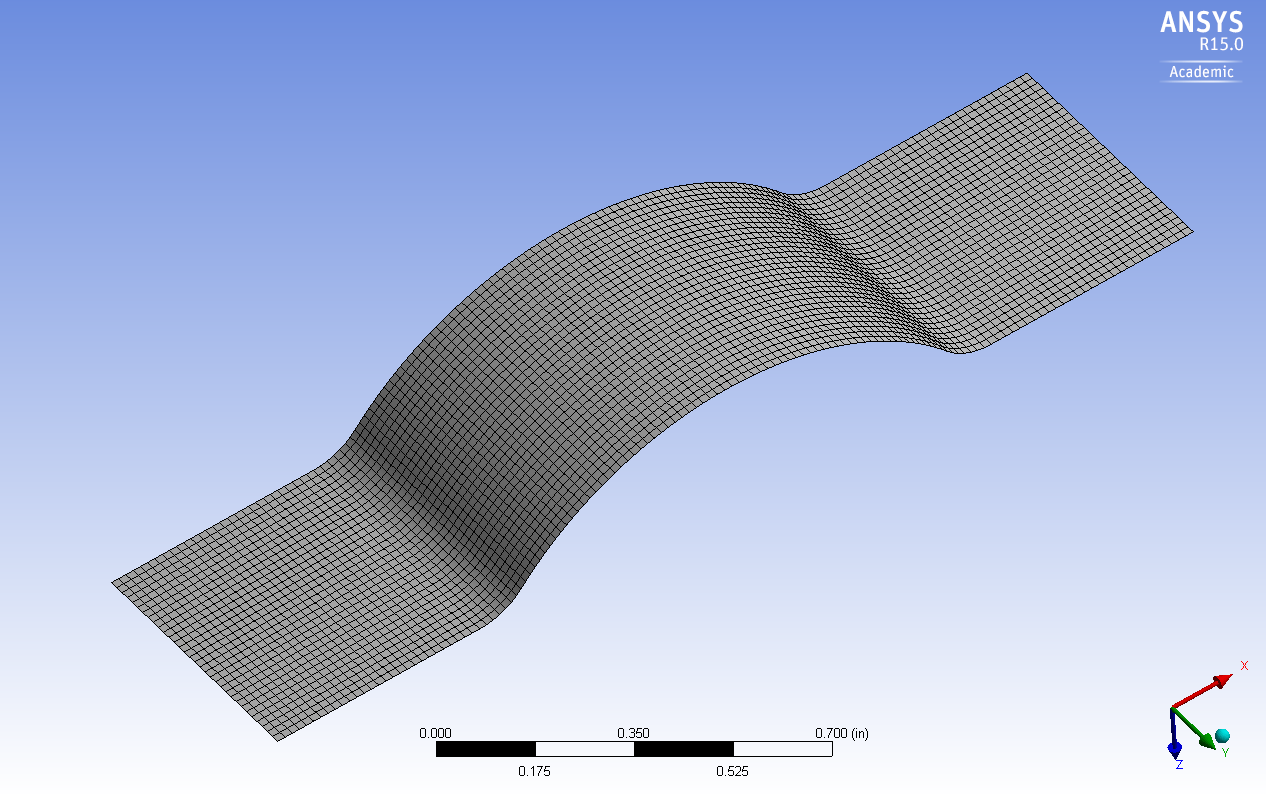
\includegraphics[width=1\textwidth]{./figures/fea/fea-mechanical-mesh-surface}
\caption{An overview of the mesh applied in \textit{ANSYS Mechanical}.}
\label{fig:fea-mechanical-mesh-surface}
\end{figure}

\begin{figure}[htp]
\centering
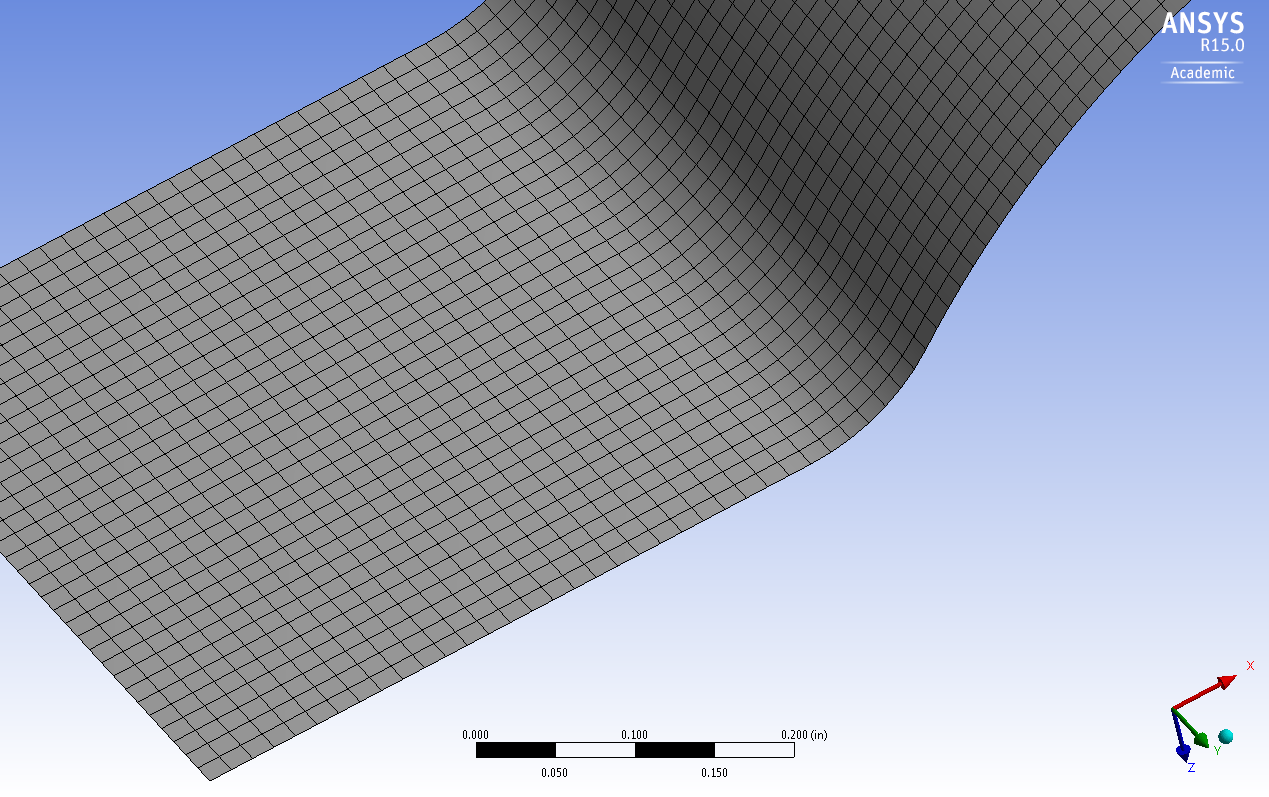
\includegraphics[width=1\textwidth]{./figures/fea/fea-mechanical-mesh-closeup}
\caption{A close-up of the mesh showing its size dependency based on feature geometry.}
\label{fig:fea-mechanical-mesh-closeup}
\end{figure}

\begin{figure}[htp]
\centering
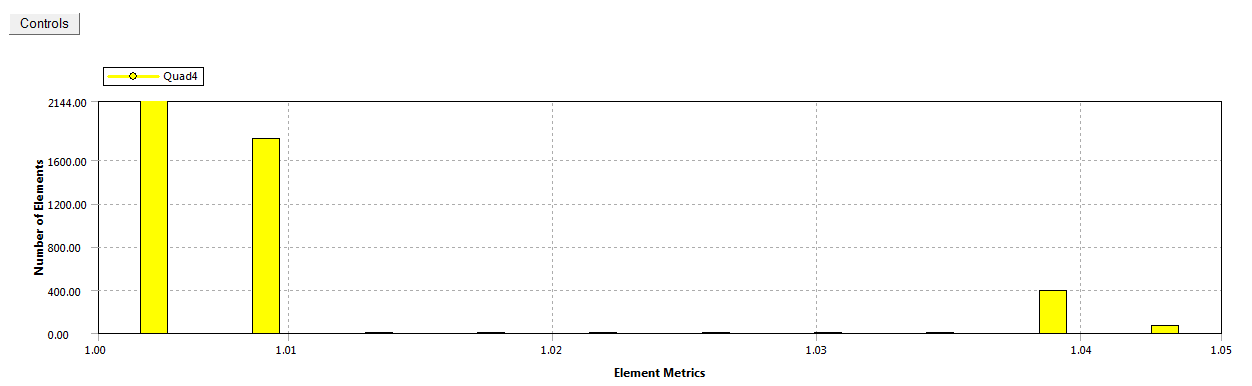
\includegraphics[width=1\textwidth]{./figures/fea/fea-mechanical-mesh-metrics-histogram}
\caption{A histogram of the aspect ratio of mesh elements.}
\label{fig:fea-mechanical-mesh-metrics-histogram}
\end{figure}

\begin{figure}[htp]
\centering
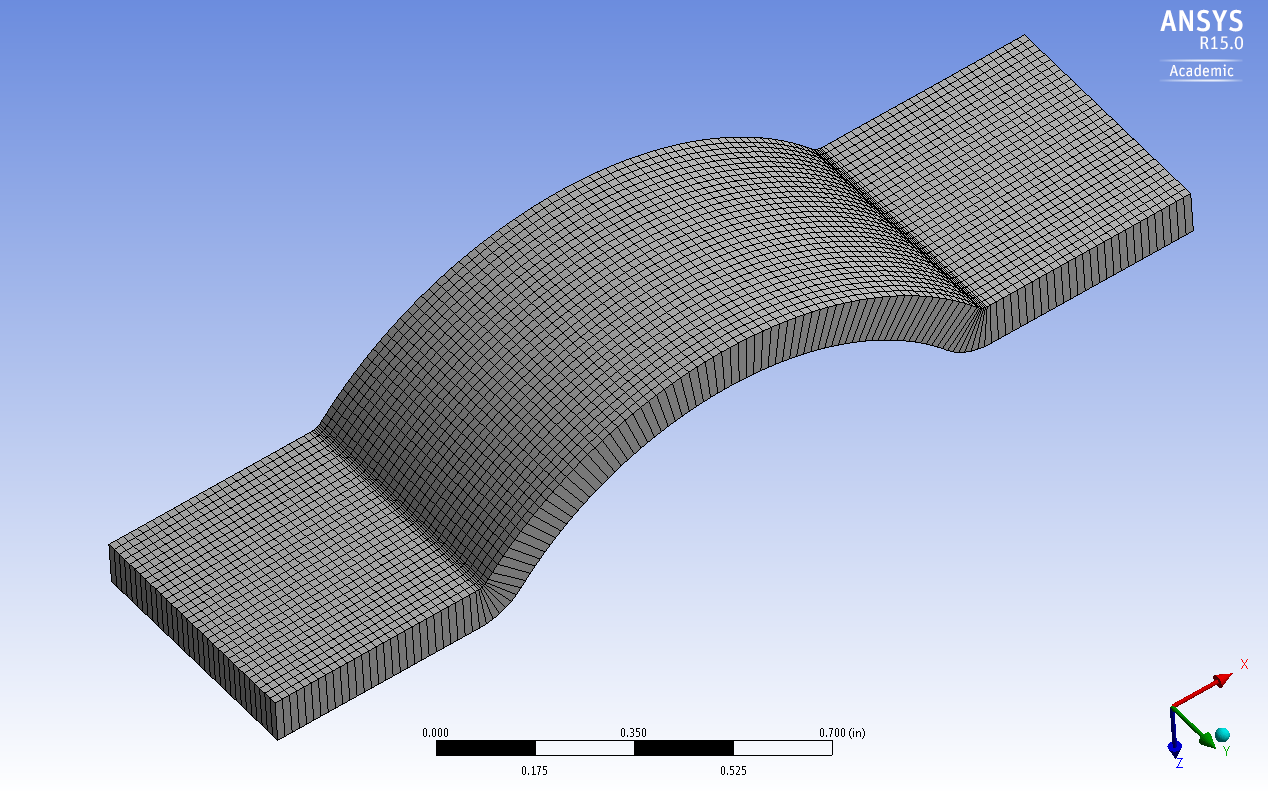
\includegraphics[width=1\textwidth]{./figures/fea/fea-mechanical-mesh-thick-shell}
\caption{The mesh as viewed when the shell elements are given a thickness.}
\label{fig:fea-mechanical-mesh-thick-shell}
\end{figure}


\clearpage

\subsection{ACP Setup}

\subsubsection{Mesh}

\indent

Figure~\ref{fig:fea-acp-mesh-overview} shows the meshed surface model after import into ACP. While not directly displayed in ACP, the loads and boundary conditions previously applied are still saved and act on the model.\\

\begin{figure}[htp]
\centering
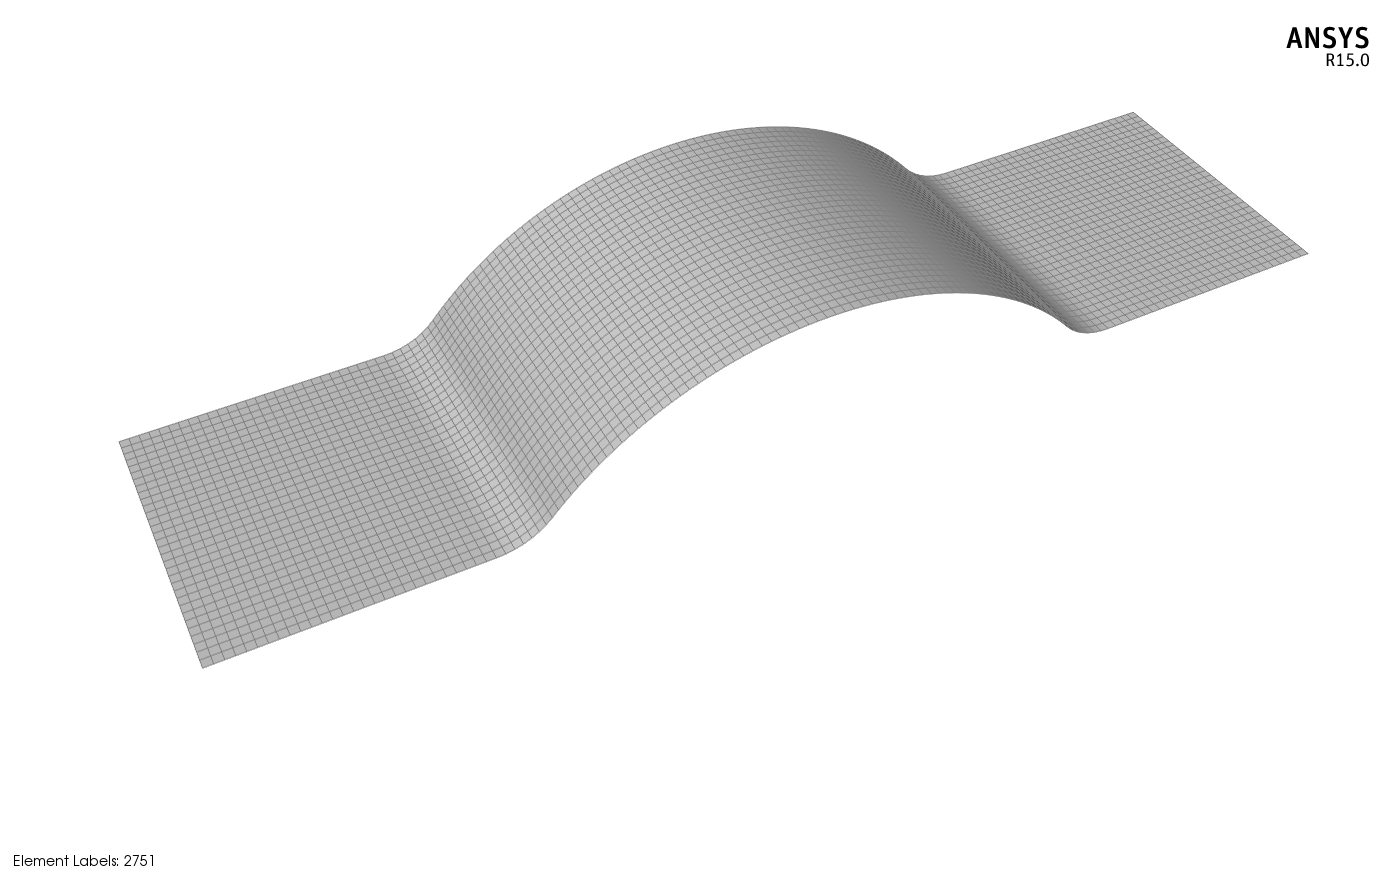
\includegraphics[width=1\textwidth]{./figures/fea/fea-acp-mesh-overview}
\caption{The mesh imported from \textit{ANSYS Mechanical} into \textit{ACP}.}
\label{fig:fea-acp-mesh-overview}
\end{figure}

\clearpage

\subsubsection{Control Tree}

\indent

Figure~\ref{fig:fea-acp-tree} shows ACP's configuration tree (all of the options availabe in setup). For this analysis \emph{Fabric Properties}, \emph{Stackup Properties}, \emph{Oriented Element Sets}, \emph{Modeling Plys}, and \emph{Solid Body Representations} were used.\\

\begin{figure}[htp]
\centering
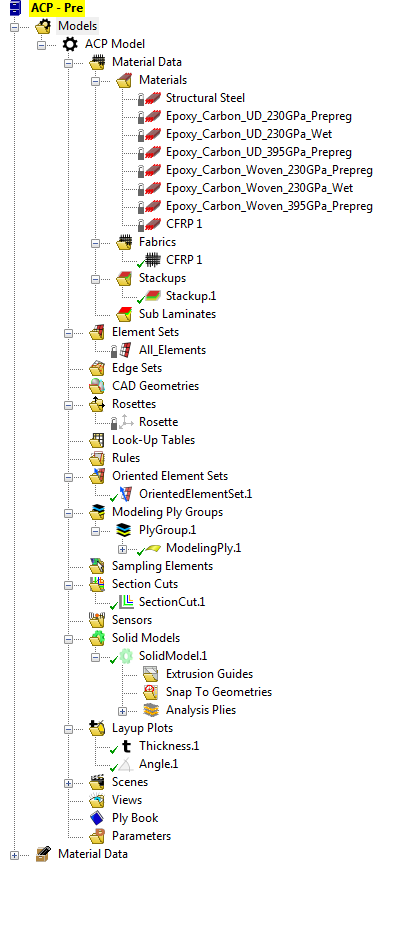
\includegraphics[width=0.25\textwidth]{./figures/fea/fea-acp-tree}
\caption{\textit{ACP}'s configuration tree.}
\label{fig:fea-acp-tree}
\end{figure}

\clearpage

\subsubsection{Fabric Properties}

\indent

Fabric properties are shown in Figure~\ref{fig:fea-acp-fabric-prorties-general}. On the general tab, the material must be selected. In this case, CFRP 1, which has the material properties listed above was selected. A thickness of one ply, or layer, is also assigned. In this case 0.4 micrometers is used. For designs in industry, pricing values can also be assigned here (and a net price can be accessed once the model is complete), but was ignored for the purpose of this FEA study. Figure~\ref{fig:fea-acp-fabric-properties-polar} shows the analysis tab with polar properties enabled. Because this is a UD CFRP specimen, polar properties must be enabled to obtain realistic results. If the speciment contained multiple layers, each layer with parrallel fibers, with each layer set perpendicular to the ones above and below it, polar properties are not necessary since the aggregate part would not be considered orthotropic.\\

\begin{figure}[htp]
\centering
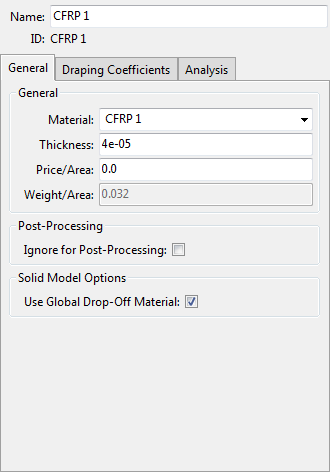
\includegraphics[width=0.5\textwidth]{./figures/fea/fea-acp-fabric-prorties-general}
\caption{General fabric proprerties used for FEA.}
\label{fig:fea-acp-fabric-prorties-general}
\end{figure}

\begin{figure}[htp]
\centering
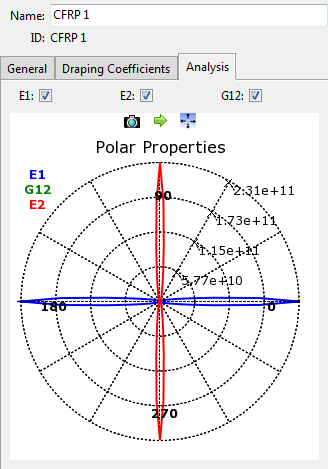
\includegraphics[width=0.5\textwidth]{./figures/fea/fea-acp-fabric-properties-polar}
\caption{Orthotropic fabric properites plotted in polar coordinates.}
\label{fig:fea-acp-fabric-properties-polar}
\end{figure}

\clearpage

\subsubsection{Stackup Properties}

\indent

Similarly, Figure~\ref{fig:fig:fea-acp-stackup-proprties} shows polar properties enabled for the analysis. Stackup reference a fabric and allow the user to combine multiple fabrics into one stack. For example, one could create a stackup with involved one type of prepreg layed ontop of another. However, this feature was not used in this FEA study.

\begin{figure}[htp]
\centering
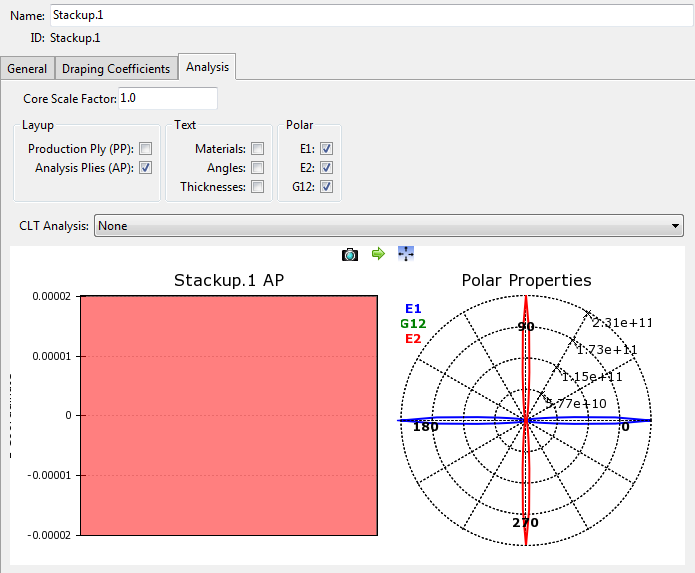
\includegraphics[width=0.5\textwidth]{./figures/fea/fea-acp-stackup-proprties}
\caption{Stackup proprerties used for FEA.}
\label{fig:fea-acp-stackup-proprties}
\end{figure}

\clearpage

\subsubsection{Oriented Elements Properties}

\indent

In order to set a reference direction and create fiber orientations, an oriented element set was created. All existing mesh elements were selected for this set. The reference direction was chosen to be aligned with the positive x axis and placed at the origin. Figure~\ref{fig:fea-acp-oriented-element-properties} shows these settings. With the reference direction established, Figure~\ref{fig:fea-acp-reference-direction} displays the refernece vector (yellow) on each element. Note that they are all parallel, which is necessary for the UD CFRP model. The x-direction of the orthotropic material automatically aligns with the reference vector in each element. Subsequently, the fiber orientation vector can be viewed (green) can be seen in Figure~\ref{fig:fea-acp-fiber-direction}. Normal vectors are also associated with each element to define the direction in which layers are offset and to define y and z material directions. Because the y and z material properties for the CFRP are treated as constant, the orientation of the normal vectors were not altered from their default orientations.\\

\begin{figure}[htp]
\centering
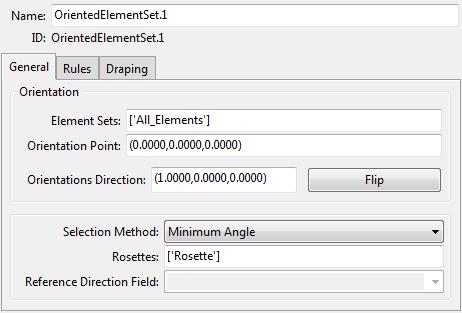
\includegraphics[width=0.5\textwidth]{./figures/fea/fea-acp-oriented-element-properties}
\caption{Oriented element properties used to establish a reference direction.}
\label{fig:fea-acp-oriented-element-properties}
\end{figure}

\begin{figure}[htp]
\centering
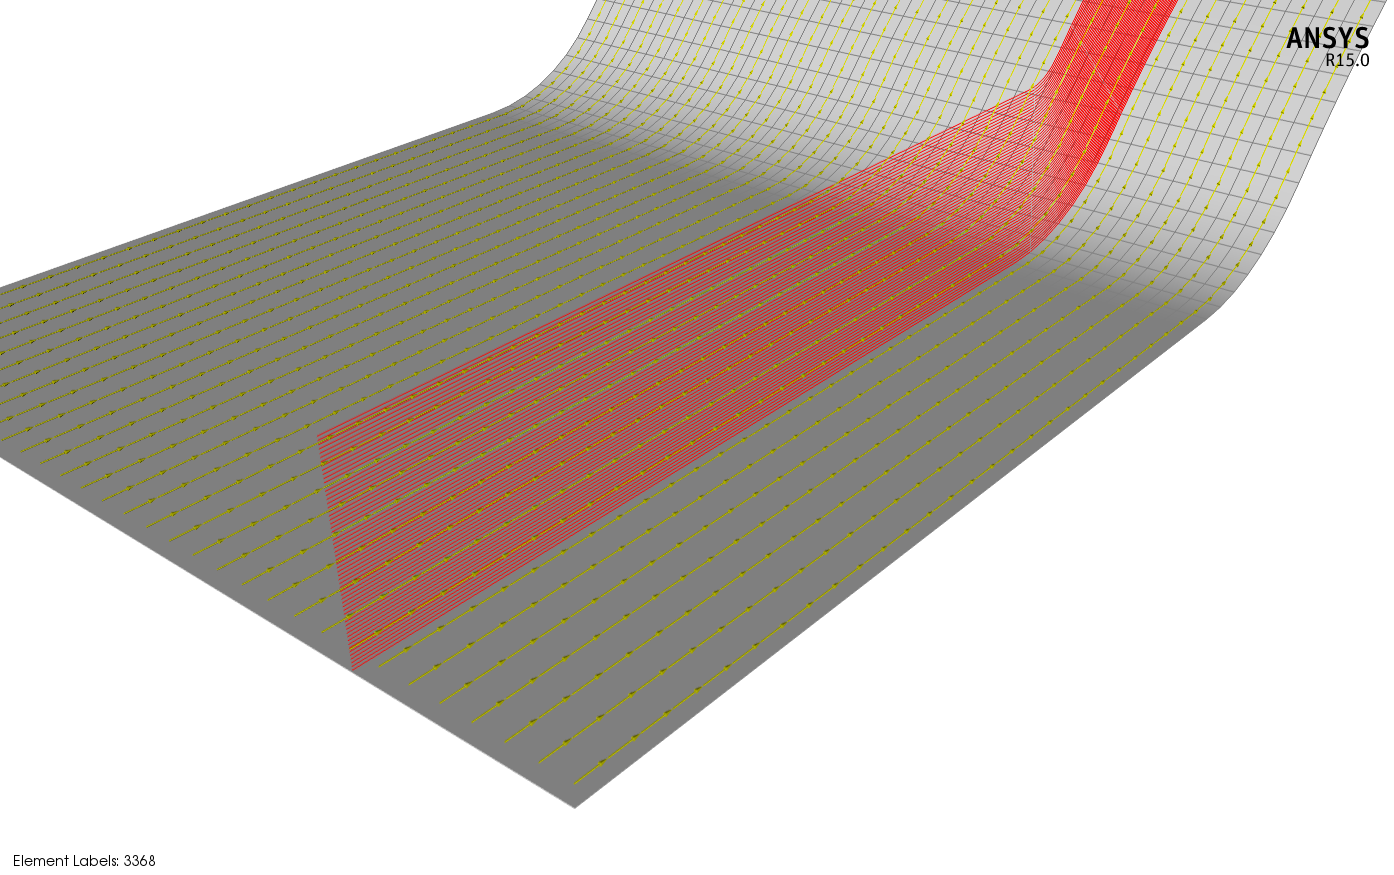
\includegraphics[width=1\textwidth]{./figures/fea/fea-acp-reference-direction}
\caption{Reference direction vector displayed in the finite element model.}
\label{fig:fea-acp-reference-direction}
\end{figure}

\begin{figure}[htp]
\centering
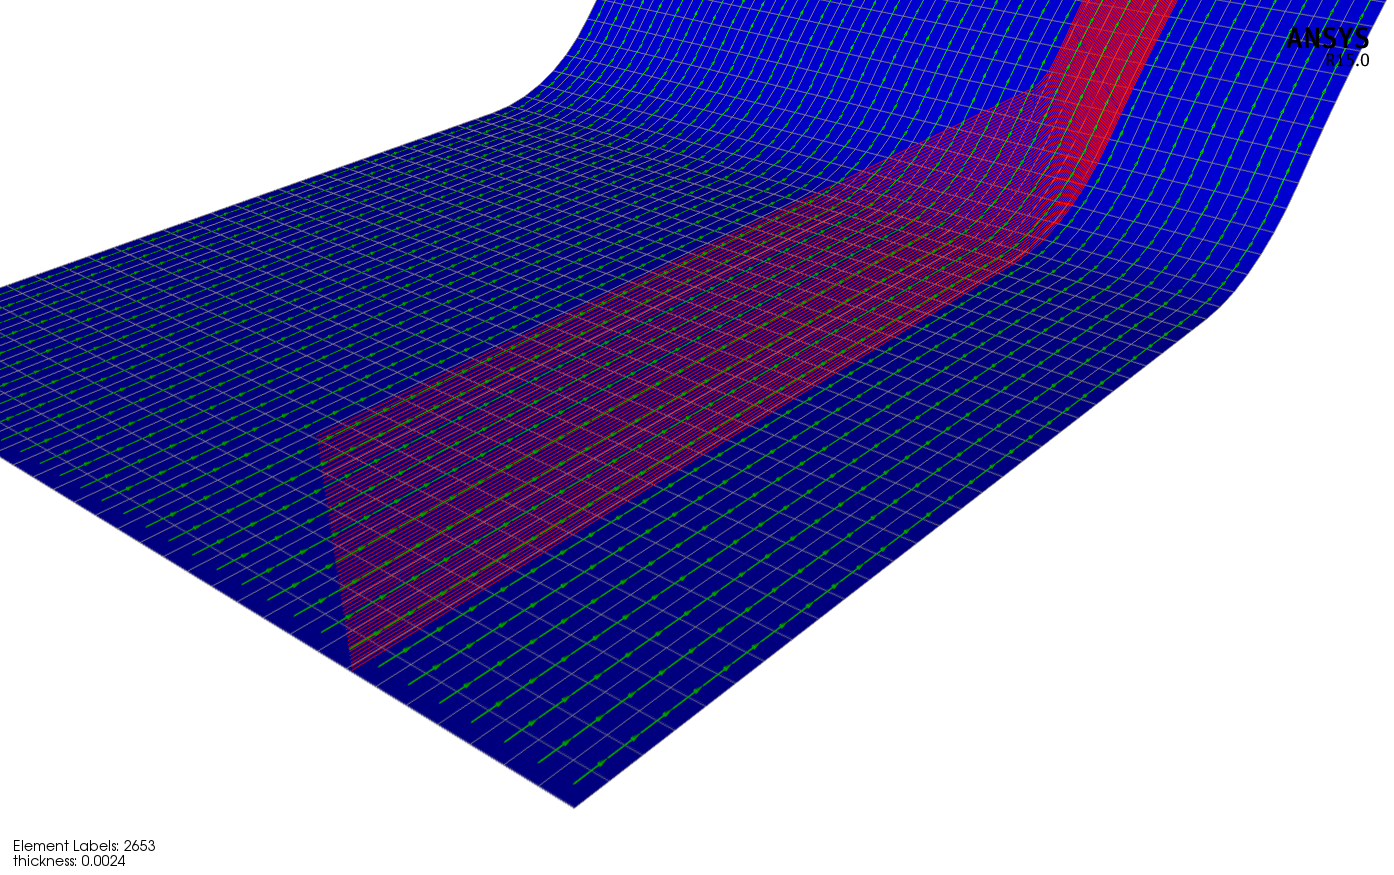
\includegraphics[width=1\textwidth]{./figures/fea/fea-acp-fiber-direction}
\caption{Fiber direction vector displayed in the finite element model.}
\label{fig:fea-acp-fiber-direction}
\end{figure}

\clearpage

\subsubsection{Modeling Plys}

\indent

As shown in Figure~\ref{fig:fea-acp-modeling-ply-properties}, modeling plys reference and existing stack up and propogate it for a number of layers. For this study, 60 layers were used to achieve the desired part thickness. Once the number of layers is set, a scalable section view is made visible, which is shown in red in Figure~\ref{fig:fea-acp-ply-scaling} showing eac ply layer.\\

\begin{figure}[htp]
\centering
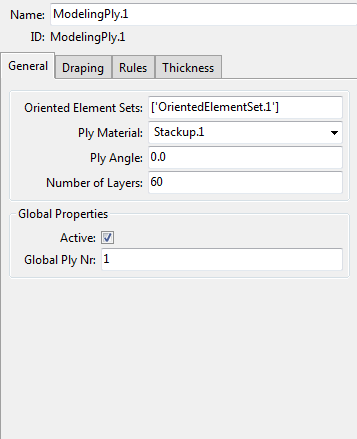
\includegraphics[width=0.5\textwidth]{./figures/fea/fea-acp-modeling-ply-properties}
\caption{Ply properties used for FEA.}
\label{fig:fea-acp-modeling-ply-properties}
\end{figure}

\begin{figure}[htp]
\centering
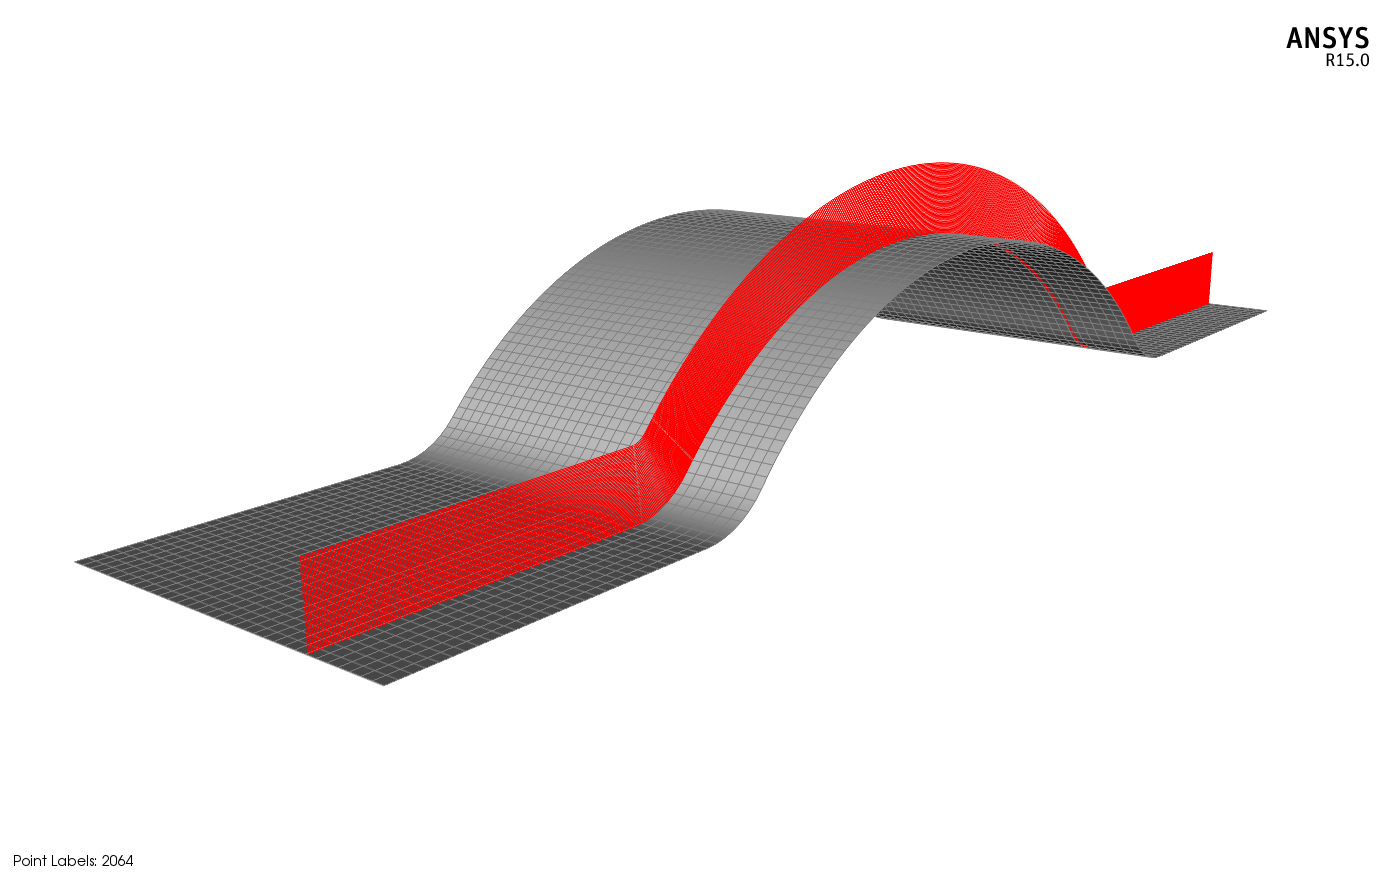
\includegraphics[width=1\textwidth]{./figures/fea/fea-acp-ply-scaling}
\caption{A ply scaling representation of the composite finitie element model.}
\label{fig:fea-acp-ply-scaling}
\end{figure}

\clearpage

\indent

The plys can also be represented as a solid body. Figure~\ref{fig:fea-acp-solidmodel-mesh} shows an overview of this display state while Figure~\ref{fig:fea-acp-solidmodel-closeup} is a closeup of an edge where ply layers are clearly visible. In addition to being a display state, solid body representation also allows ACP to perform the analysis using more rigorous 3D states of stress rather than 2D.\\

\subsubsection{Solid Body Representation}

\begin{figure}[htp]
\centering
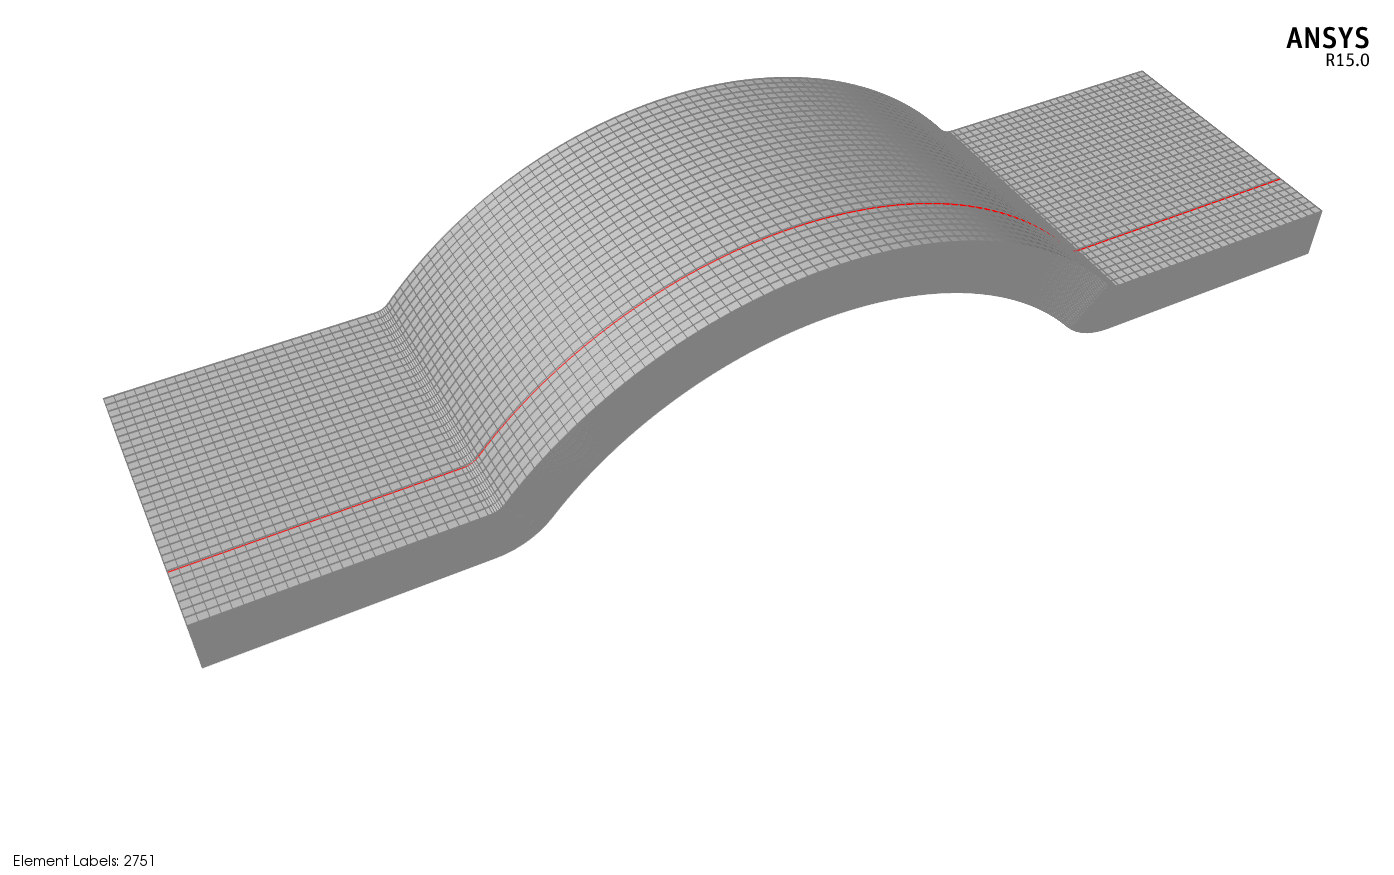
\includegraphics[width=1\textwidth]{./figures/fea/fea-acp-solidmodel-mesh}
\caption{Mesh overview of the composite model in \textit{ACP} with a solid-body display state applied.}
\label{fig:fea-acp-solidmodel-mesh}
\end{figure}

\begin{figure}[htp]
\centering
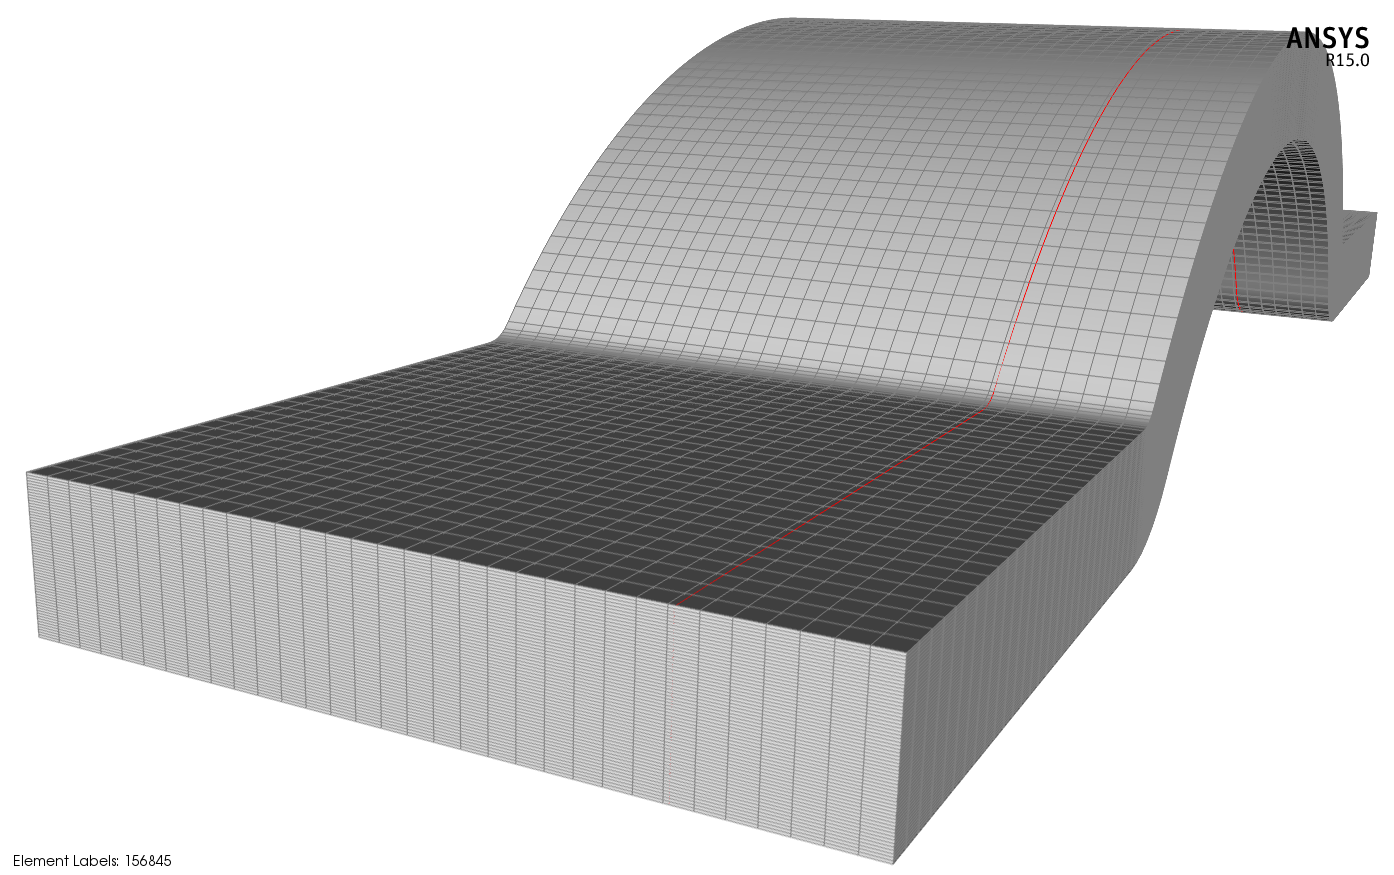
\includegraphics[width=1\textwidth]{./figures/fea/fea-acp-solidmodel-closeup}
\caption{Mesh overview of the composite model in \textit{ACP} with a solid-body display state applied.}
\label{fig:fea-acp-solidmodel-closeup}
\end{figure}

\clearpage

\subsection{Failure Criteria}

\indent

As mentioned, Puck's failure critera was used for this finite element analysis, and is configured in post-processing. Figure~\ref{fig:fea-acp-failure-criteria-definition} shows the window where Puck is selected. Although it was not done in this study, multiple failure criteria can be configured for any analysis. Figure~\ref{fig:fea-acp-puck-failure-criterion} displays the specific options selected for this configuration. Note the default Puck constants that were defined with the CFRP material could be altered in this window. For this analysis, Puck's constants were left untouched, the model solved using a 3D state of stress which access fiber stress data to determine its impact on IFF scenarios, and ignores fiber failure options since tensile test shows that the matrix material of this filament clearly fails before the fiber.\\

\begin{figure}[htp]
\centering
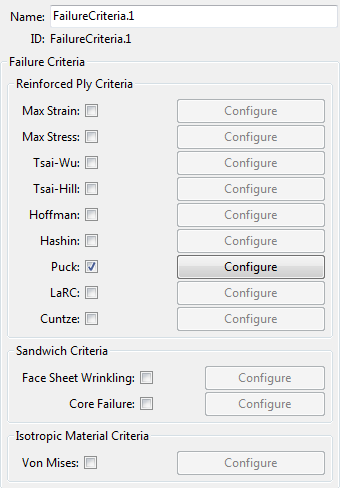
\includegraphics[width=0.5\textwidth]{./figures/fea/fea-acp-failure-criteria-definition}
\caption{Composite failure criteria available in \textit{ACP}.}
\label{fig:fea-acp-failure-criteria-definition}
\end{figure}

\begin{figure}[htp]
\centering
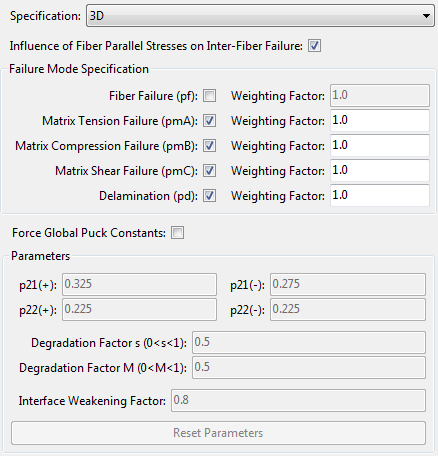
\includegraphics[width=0.5\textwidth]{./figures/fea/fea-acp-puck-failure-criterion}
\caption{The Puck failure criterion properties applied to the finite element model.}
\label{fig:fea-acp-puck-failure-criterion}
\end{figure}

\clearpage

\subsection{Solid Body FEA Comparison}

\indent

For comparison, and model validation, solid-body FEA studies of ABS and aluminum were performed. Ideally the studies would show that the CFRP ACP model was stronger than ABS and weaker than aluminum, while stiffer than ABS and nearly as stiff and aluminum (given the same loading conditions). The setup of these finite element analysis are detailed here. Results are also graphically displayed but are discussed in the main body of this report.

\subsubsection{Physics Models}

\indent

A static structural analysis was performed in \emph{ANSYS} mechanical using solid body geometry imported from \emph{SolidWorks}. ACP was not utilized for the ABS case because it is only meant for composite materials, which pure ABS is not. Subsequently, while that software package could locate delamination failures, which would be of interest in an FDM part, the results would be false and incorrect because the package would be using composite failure criteria. \\

\subsubsection{Geometry}

Figure~\ref{fea-body-geometry} shows a \emph{SolidWorks} drawings of the geometry imported into \emph{ANSYS Mechanical}.

\begin{figure}[htp]
\centering
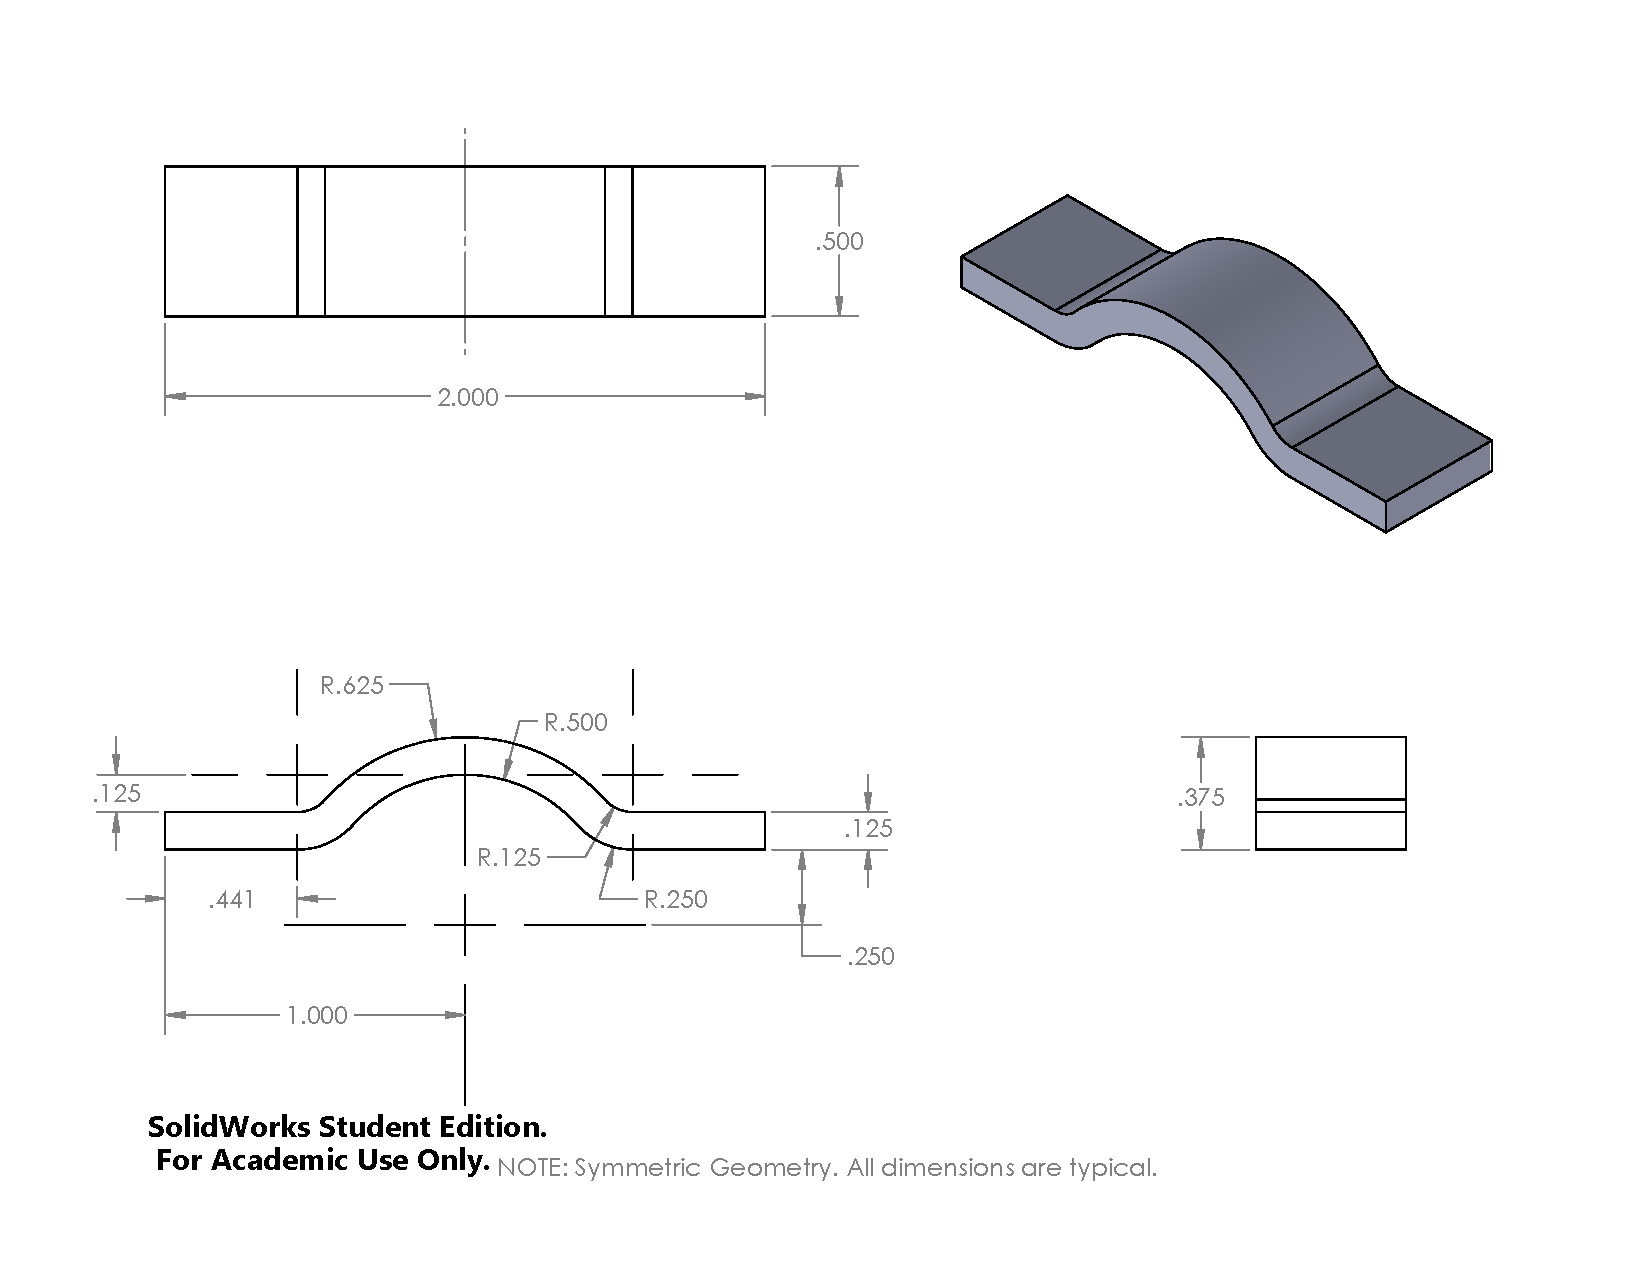
\includegraphics[width=1\textwidth]{./figures/fea/fea-body-geometry}
\caption{A \emph{SolidWorks} drawing of the solid body used for the comparison FEA.}
\label{fig:fea-body-geometry}
\end{figure}

\clearpage

\subsubsection{Material Properties}

\indent

Properties for the aluminum analysis were pulled from the materials library for aluminum alloy within \emph{ANSYS}. ABS is not included within the library and had to be input as a new material using the previously tabulated ABS data. Table~\ref{tab:abs-properties} lists these values.\\

\begin{table}[htp]
    \centering
    \begin{tabular}{lcc}
        Property & Value & Unit \\ \hline
        
        Density & 1024 & kg m$^{-3}$\\ 
        Young's Modulus & 1.8E+06 & Pa\\
        Poisson's Ratio & 0.35 & \\
        Bulk Modulus & 2E+06 & Pa \\
        Shear Modulus & 6.67E+05 & Pa\\
        
    \end{tabular}
    \caption{ABS material properties used for a standard finite element analysis.}
    \label{tab:abs-properties}
\end{table}

\clearpage

\subsubsection{Mesh}

\indent 1/64 inch

Figure~\ref{fig:fea-solid-mesh-overview} shows an overview of the mesh used to descritize the solid geometry while Figure~\ref{fig:fea-solid-mesh-closeup} shows a closeup of the mesh on the smallest geometric feature. A global mesh sizing constraint (1/64 inches) and sweep method were used to generate this mesh. While this mesh is significantly finer than the one in ACP, mesh sensitivity studies (increasing mesh resolution until stress values stop increasing with each increment and settle) deemed that extra resolution was necessary. Subsequently, aspect ratio statistics in Figure~\ref{fig:fea-solid-mesh-metrics} show good statistics (all elements below 3).\\

\begin{figure}[htp]
\centering
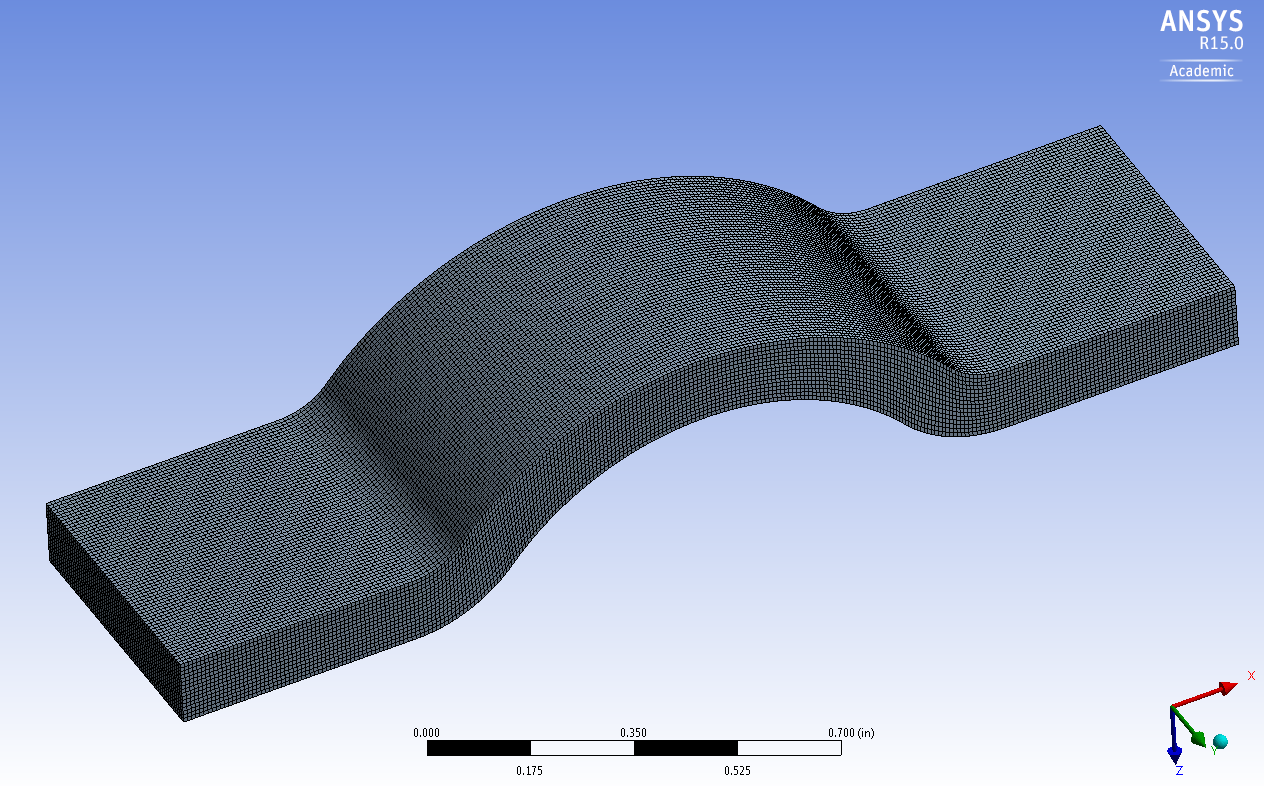
\includegraphics[width=1\textwidth]{./figures/fea/fea-solid-mesh-overview}
\caption{An overview of the mesh used for the standard FEA.}
\label{fig:fea-solid-mesh-overview}
\end{figure}

\begin{figure}[htp]
\centering
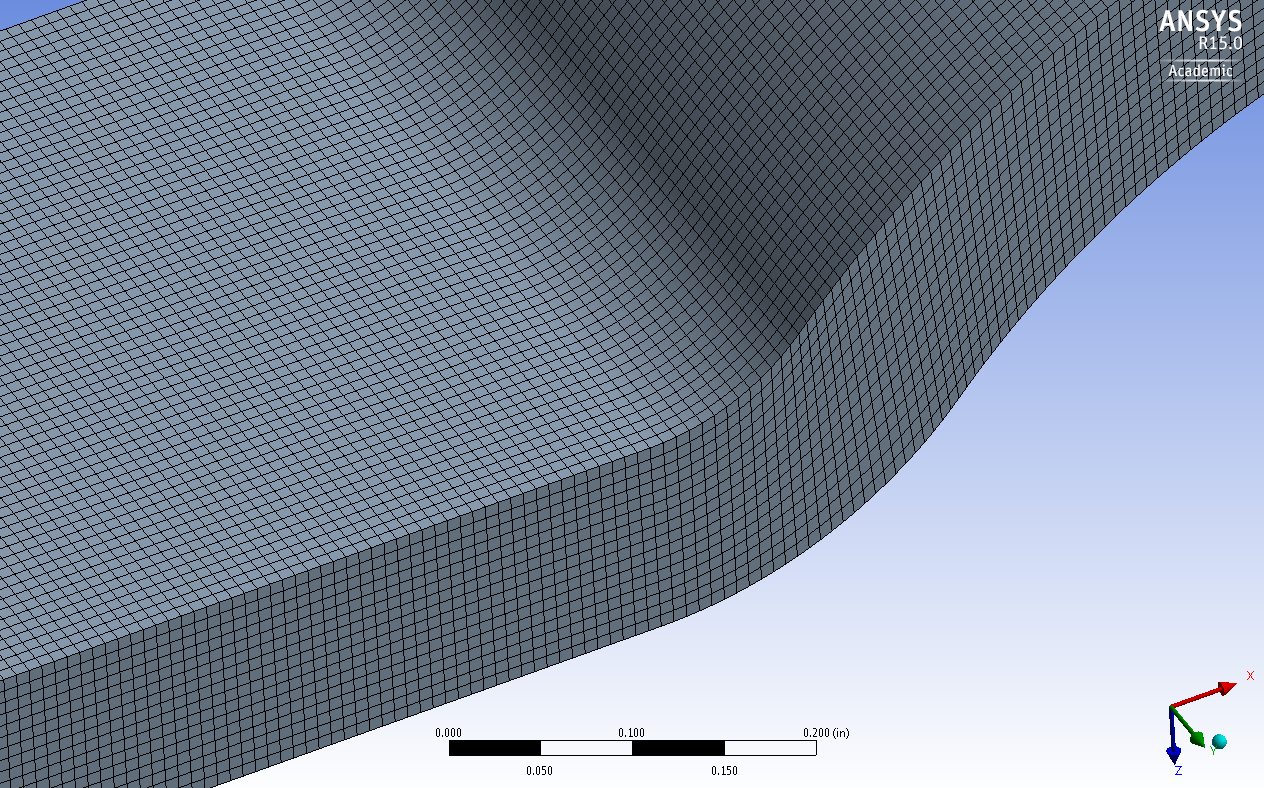
\includegraphics[width=1\textwidth]{./figures/fea/fea-solid-mesh-closeup}
\caption{A close-up of the mesh used for the standard FEA.}
\label{fig:fea-solid-mesh-closeup}
\end{figure}

\begin{figure}[htp]
\centering
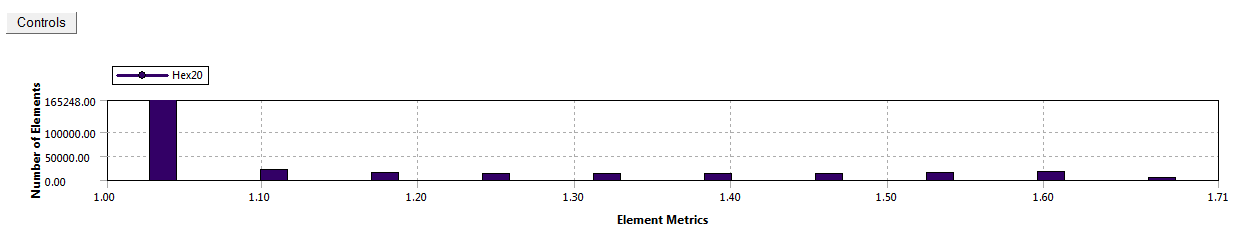
\includegraphics[width=1\textwidth]{./figures/fea/fea-solid-mesh-metrics}
\caption{Mesh statistics for the solid model FEA.}
\label{fig:fea-solid-mesh-metrics}
\end{figure}

\clearpage

\subsubsection{Loads and Boundary Conditions}

\indent

The same boundary conditions applied in ACP were applied to this model. Figure~\ref{fig:fea-solid-loads-bcs} and Figure~\ref{fig:fea-solid-loads-bcs-3} show the zero-displacement, fixed and force conditions that represent compression in the Instron when clamped in the jaws.\\

\begin{figure}[htp]
\centering
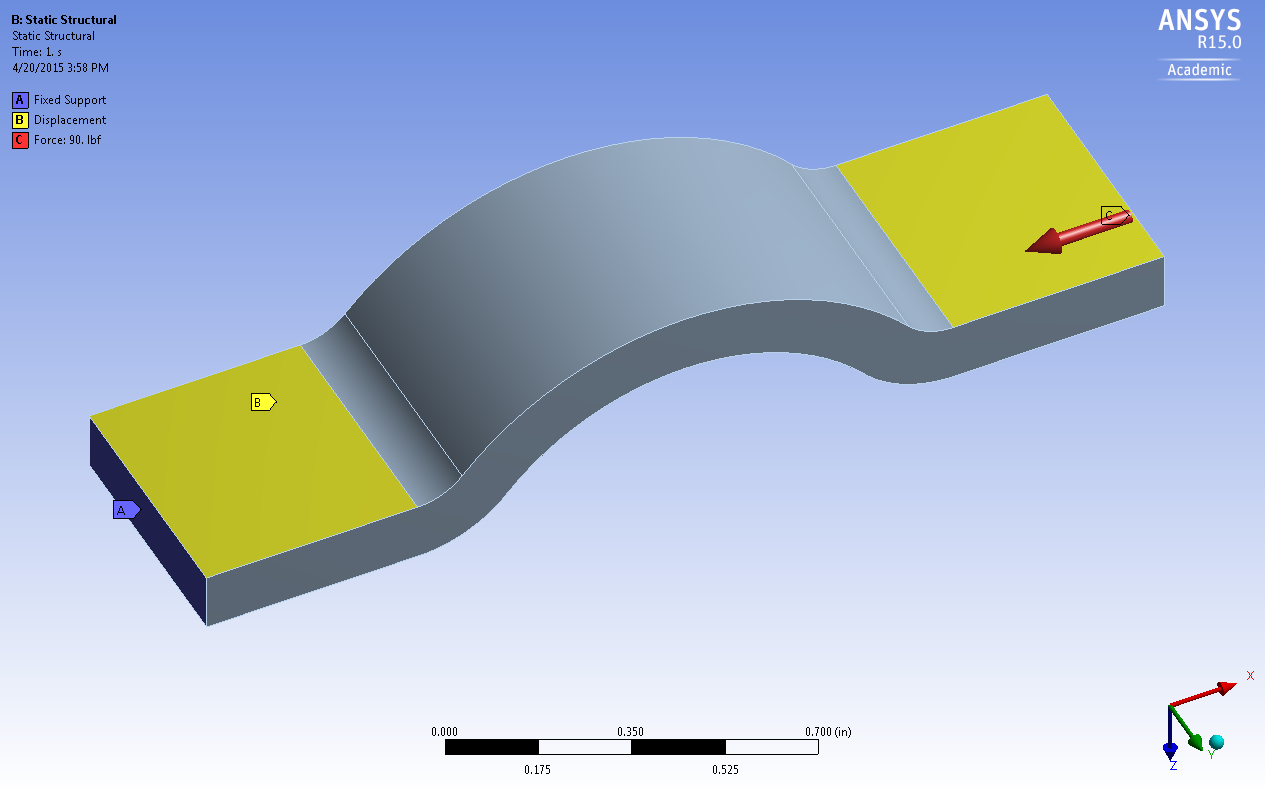
\includegraphics[width=1\textwidth]{./figures/fea/fea-solid-loads-bcs}
\caption{Loads and boundary conditions applied to the solid model fea.}
\label{fig:fea-solid-loads-bcs}
\end{figure}

\begin{figure}[htp]
\centering
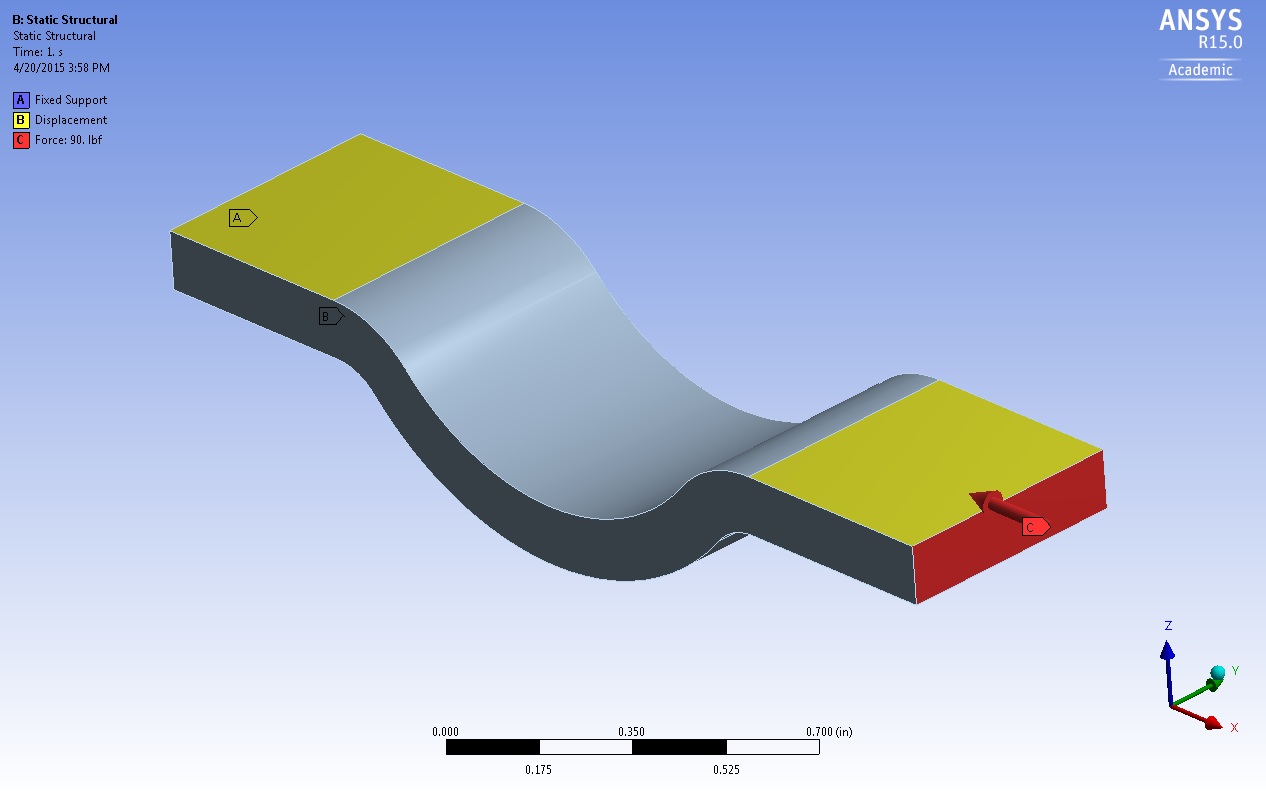
\includegraphics[width=1\textwidth]{./figures/fea/fea-solid-loads-bcs-3}
\caption{Another view of loads and boundary conditions applied to the solid model fea.}
\label{fig:fea-solid-loads-bcs-3}
\end{figure}

\clearpage

\subsubsection{Results}

%%% ABS

\indent

Figure~\ref{fig:fea-solid-vms-top} and Figure~\ref{fig:fea-solid-vms-bottom} are contour plots of Von Mises stress distributions the ABS part. Values in red exceed the ultimate flexural stress of the plastic. Note that displacement plots of ABS are not shown due to the illogical response described in the main body of this report.\\

\begin{figure}[htp]
\centering
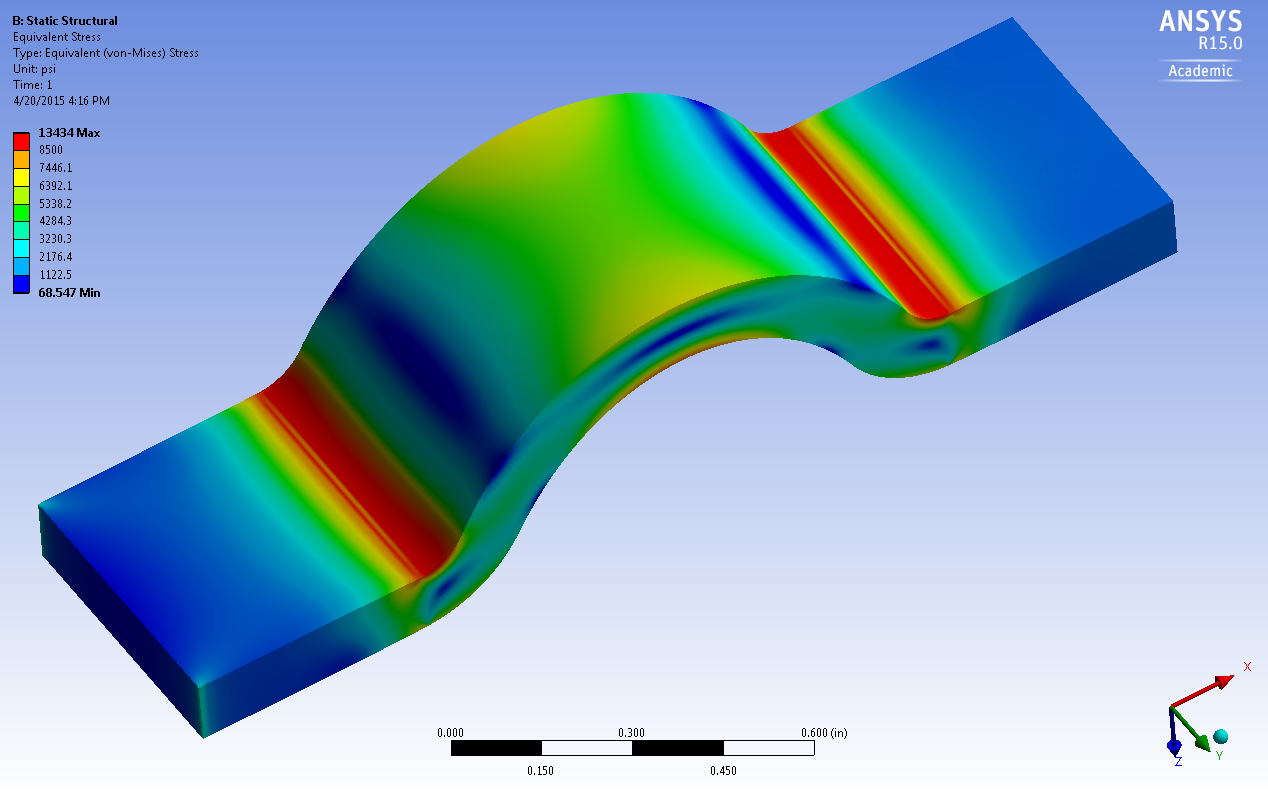
\includegraphics[width=1\textwidth]{./figures/fea/fea-solid-vms-top}
\caption{A top-isometric view of von-mises stress for a solid-body ABS analysis.}
\label{fig:fea-solid-vms-top}
\end{figure}

\begin{figure}[htp]
\centering
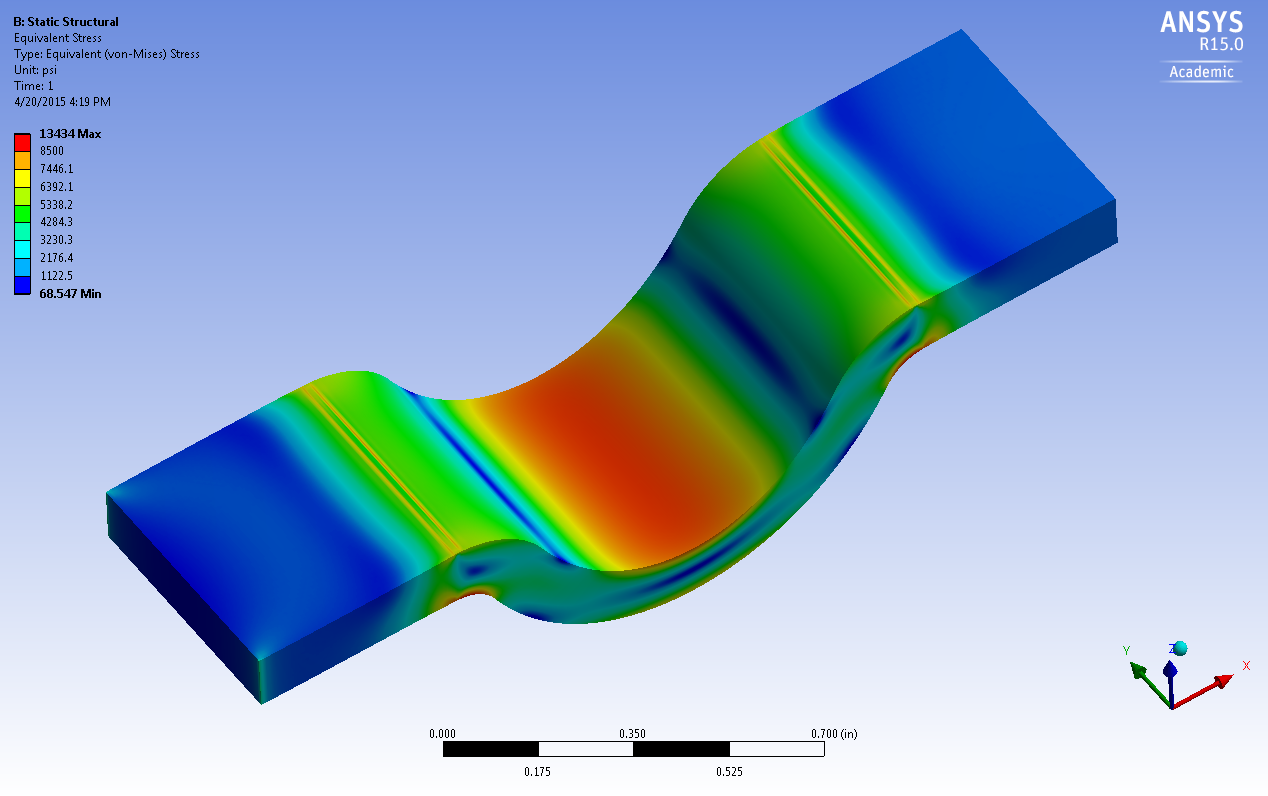
\includegraphics[width=1\textwidth]{./figures/fea/fea-solid-vms-bottom}
\caption{A bottom -isometric view of von-mises stress for a solid-body ABS analysis.}
\label{fig:fea-solid-vms-bottom}
\end{figure}

\clearpage

%%% Aluminum

Figure~\ref{fig:fea-solid-al-vms-top} and Figure~\ref{fig:fea-solid-al-vms-bottom} are contour plots of Von Mises stress distributions the aluminum part. Note that no elemenents exceed the ultimate tensile strength of aluminum (which would be shown in red). Figure~\ref{fig:fea-solid-al-def-tot} through Figure~\ref{fig:fea-solid-al-def-z} show displacement contour plots of the aluminum part.\\

%stresses

\begin{figure}[htp]
\centering
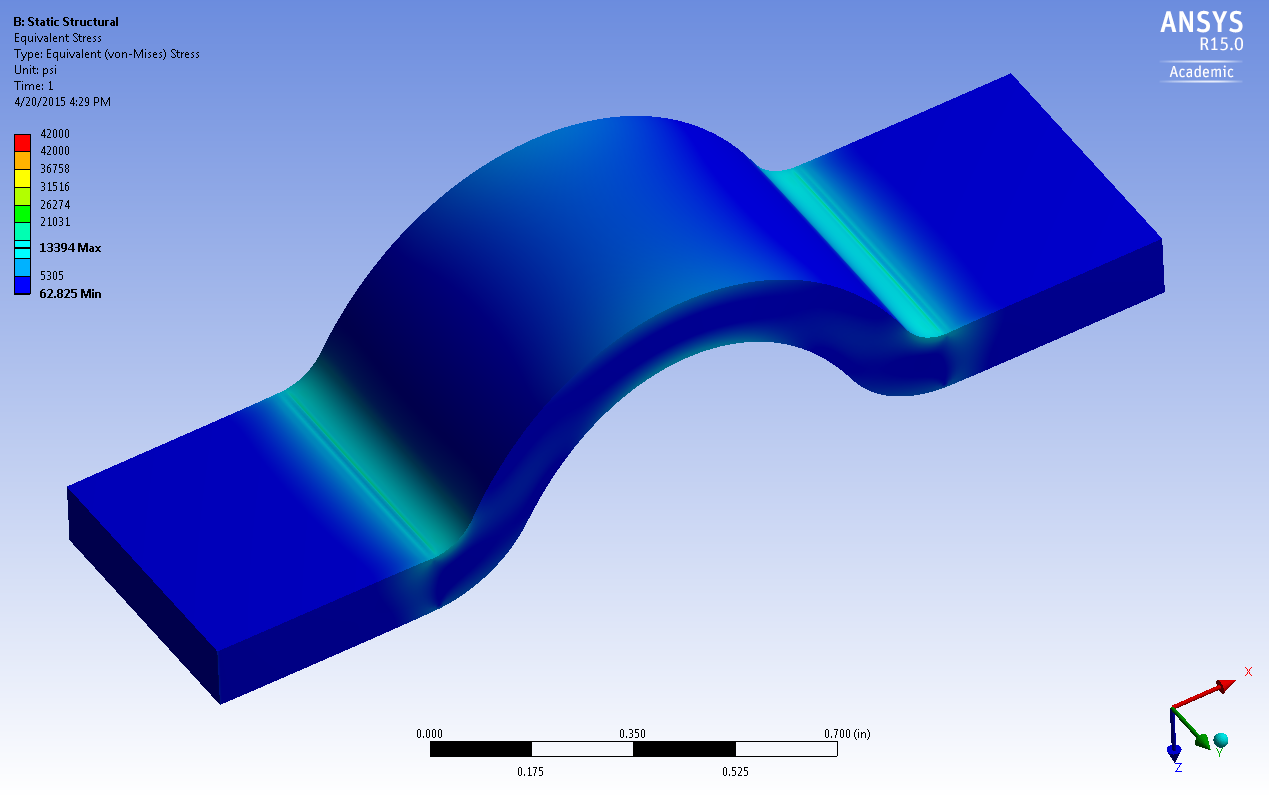
\includegraphics[width=1\textwidth]{./figures/fea/fea-solid-al-vms-top}
\caption{A top-isometric view of von-mises stress for a solid-body aluminum analysis.}
\label{fig:fea-solid-al-vms-top}
\end{figure}

\begin{figure}[htp]
\centering
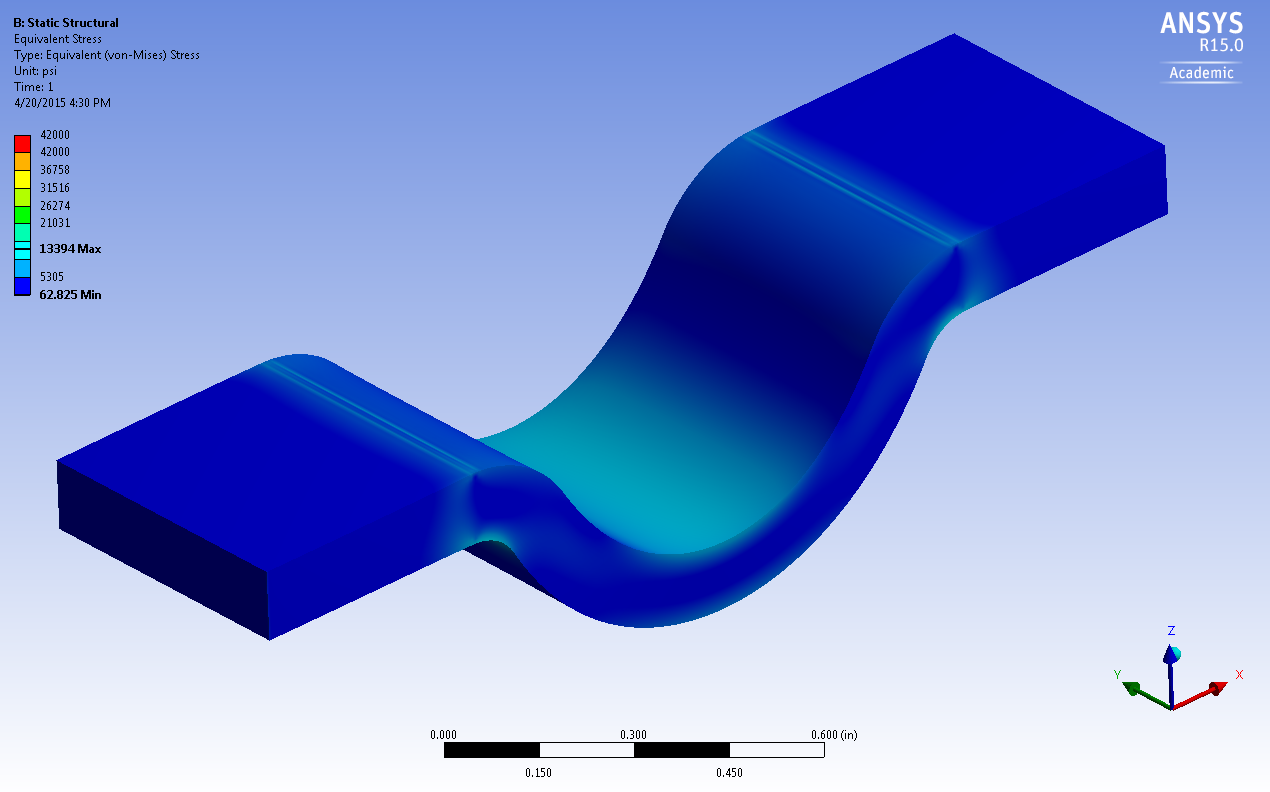
\includegraphics[width=1\textwidth]{./figures/fea/fea-solid-al-vms-bottom}
\caption{A bottom -isometric view of von-mises stress for a solid-body aluminum analysis.}
\label{fig:fea-solid-al-vms-bottom}
\end{figure}

% deformations

\begin{figure}[htp]
\centering
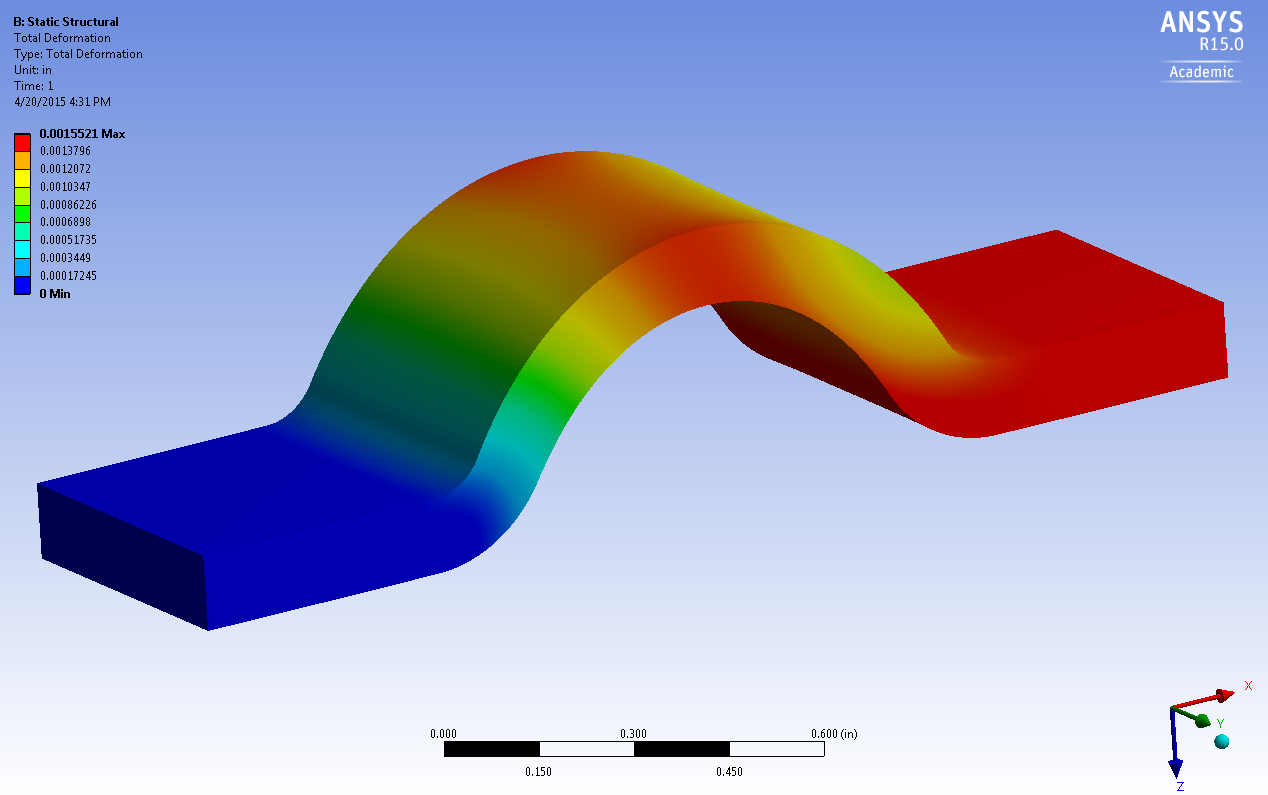
\includegraphics[width=1\textwidth]{./figures/fea/fea-solid-al-def-tot}
\caption{Total deformation from the solid-body aluminum analysis.}
\label{fig:fea-solid-al-def-tot}
\end{figure}

\begin{figure}[htp]
\centering
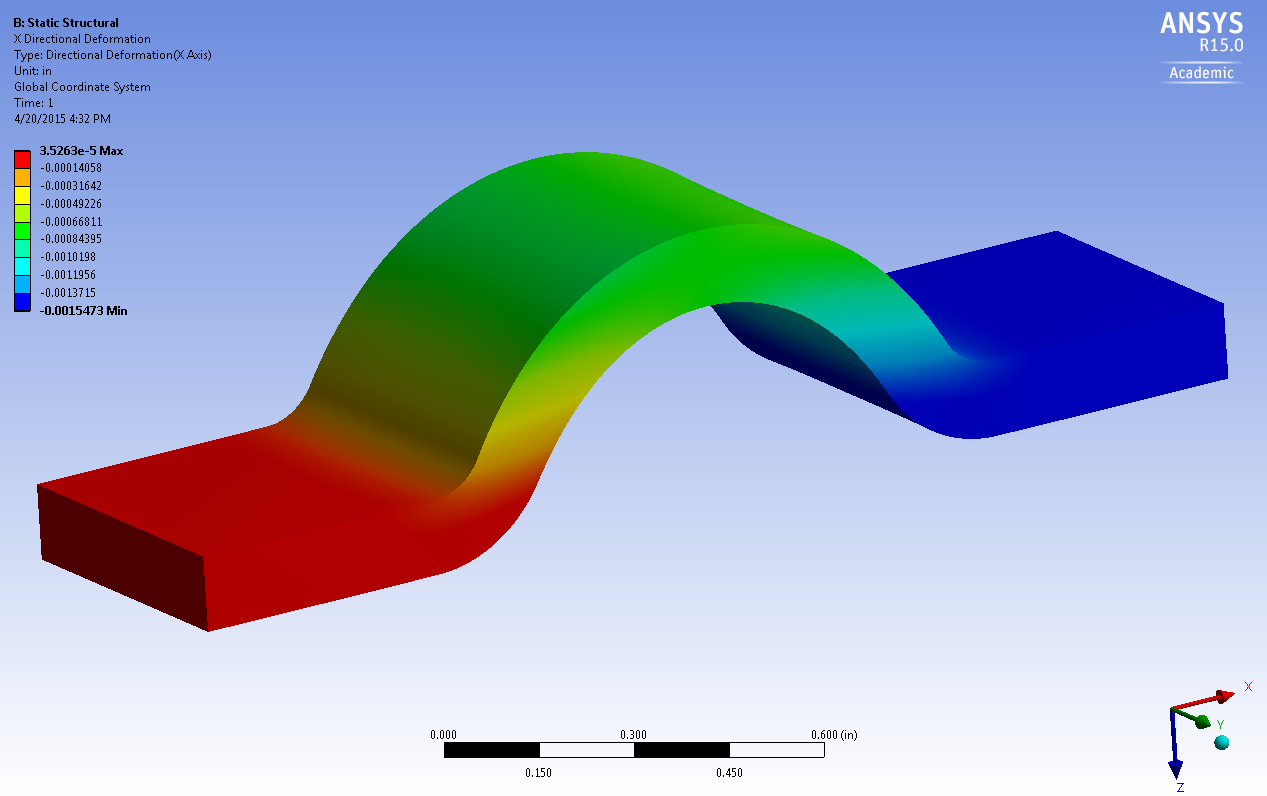
\includegraphics[width=1\textwidth]{./figures/fea/fea-solid-al-def-x}
\caption{X direction deformation from the solid-body aluminum analysis.}
\label{fig:fea-solid-al-def-x}
\end{figure}

\begin{figure}[htp]
\centering
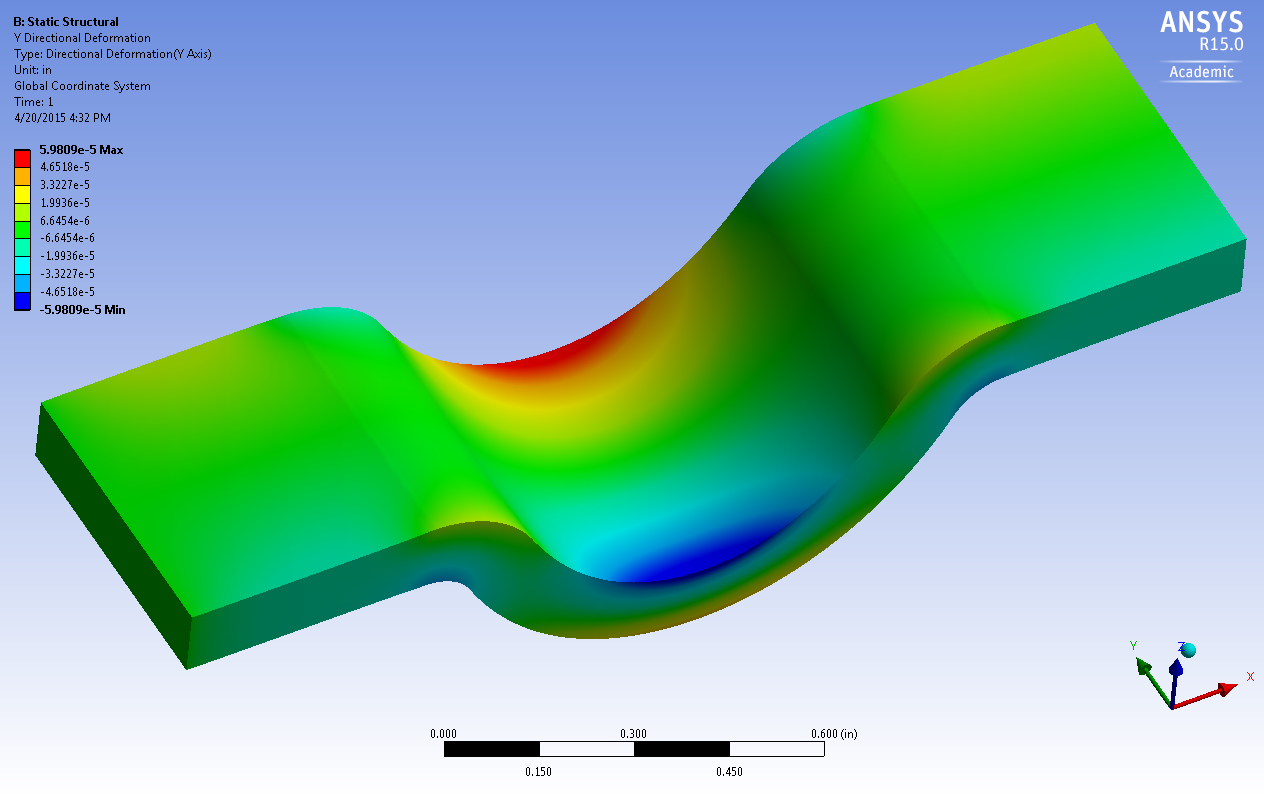
\includegraphics[width=1\textwidth]{./figures/fea/fea-solid-al-def-y}
\caption{Y direction deformation from the solid-body aluminum analysis.}
\label{fig:fea-solid-al-def-y}
\end{figure}

\begin{figure}[htp]
\centering
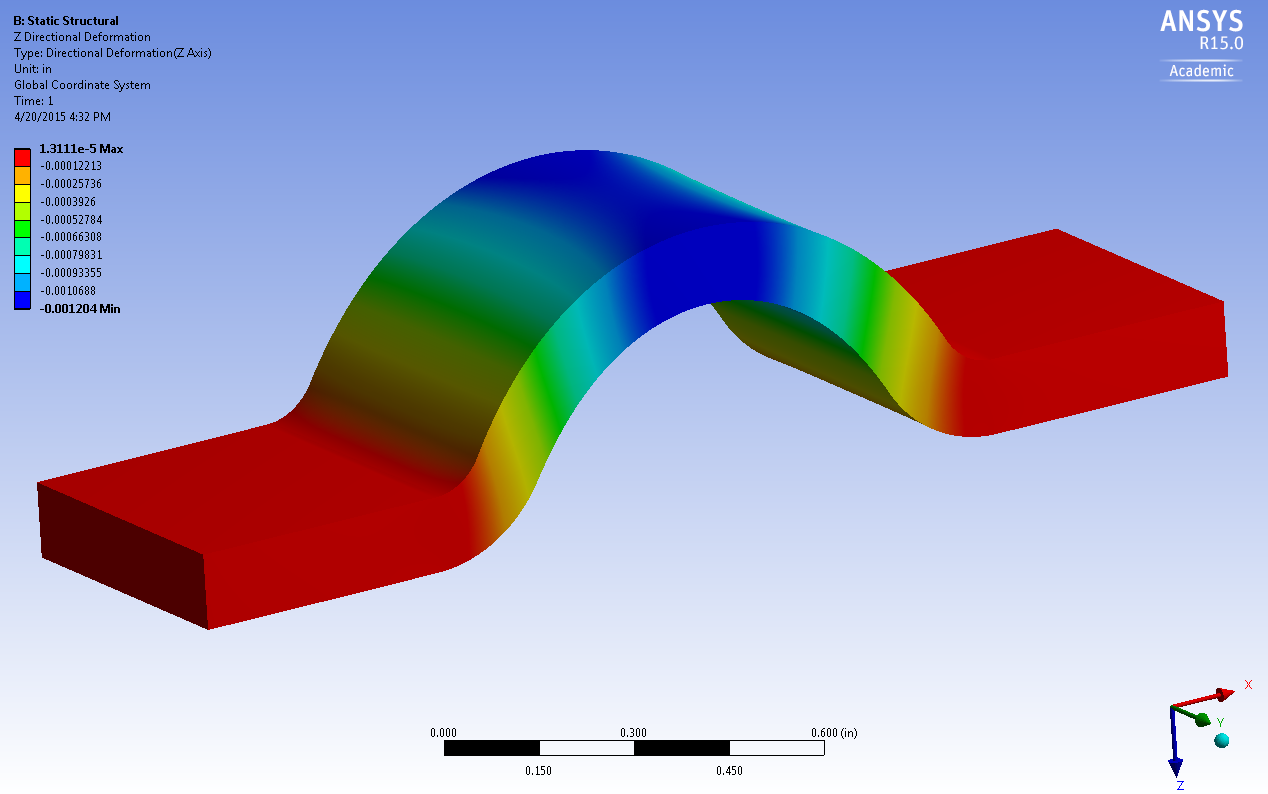
\includegraphics[width=1\textwidth]{./figures/fea/fea-solid-al-def-z}
\caption{Z direction deformation from the solid-body aluminum analysis.}
\label{fig:fea-solid-al-def-z}
\end{figure}

\clearpage

\subsection{Conclusions from FEA}

As summarized in the report body, the CFRP FDM results from ACP are logical when compared to the ABS and aluminum finite element results and are confirmed by qualitative applications of Puck's theory. Of course, without a physical printed part to experimentally test, the ACP model cannot be completely validated. Therefore, it is important going forward that printed pieces are experimentally tested and ACP setup properties are tweaked to match experimental data as closely as possible. For instance, Puck failure critera were all weighted at unity. While changing these values slightly affects the output results\footnote{Testing this only indicated that failure mode altered, never the critical ply layer.}, it is best practive to adjust the model, which potentially means changing these values, to most accurately reflect the parts physically observed failure behavior.\\

\clearpage
